%\documentclass{llncs}
\documentclass{svmult}

\usepackage{graphicx}
\usepackage{booktabs}
\usepackage{amsmath}
\usepackage[ruled,lined]{algorithm2e}
\usepackage{multirow}
\usepackage[bookmarks=false]{hyperref}
\pdfminorversion=4

\newcommand{\red}[1]{\textcolor{red}{#1}}

\hypersetup{colorlinks=true,linkcolor=black,citecolor=black}

\SetKwInput{KwData}{Global params.}

\title*{
    Testing traversability of protein tunnels with flexible ligands using motion planning
}

\author{
    Vojt\v ech Von\' asek \and 
    Barbora Kozl\'\i kov\'a  \and 
    Adam Jur\v{c}\'\i k  \and 
    David Bend\'{a}\v{r}  \and
    Martin Saska }


\institute{
    V. Von\'{a}sek, Martin Saska \at 
    Faculty of Electrical Engineering,  
Czech Technical University in Prague, 
Technick\'a 2, 166 27, Prague 6, Czech Republic
\email{vonasek@labe.felk.cvut.cz}  
\and
B. Kozl\'{\i}kov\'{a}, A. Jur\v{c}\'{\i}k \at
Faculty of Informatics,  
Masaryk University, 
Botanick\'a 68a, 602 00 Brno, \\
\and 
\inst{3}
TODO DAVID \at TODO DAVID
}


\makeindex

\def\qrand{q_{rand}}
\def\qstart{q_{start}}
\def\qinit{\qstart}
\def\qgoal{\qstart}
\def\qnear{q_{near}}
\def\qnew{q_{new}}
\def\T{\mathcal{T}}

\def\C{\mathcal{C}}
\def\CF{\mathcal{C}_{free}}
\def\CFD{{\mathcal{C}^s_{free}}}
\def\dt{d_{tunnel}}
\def\da{d_{atom}}


\def\Imax{I_{max}} %max number of iterations of RRT-based planners

\def\dist{\mathrm{dist}}
\def\dists{\mathrm{dist}_{\mathrm{s}}}

\SetKw{return}{return}

\def\VV{V_{vor}}
\def\VVA{V_{vor}^{act}}

\def\smin{s_{min}}
\def\smax{s_{max}}
\def\sdelta{{\Delta}_s}


\def\probe{r_{\mathrm{probe}}}
\def\Sprobe{S_{\mathrm{probe}}}

\def\gprobe{r_{\mathrm{out}}}
\def\Sgprobe{S_{\mathrm{out}}}


\def\CG{\mathcal{C}_{goal}}
\def\SB{\mathbf{S}_{blocking}}
\def\SS{\mathbf{S}}

\def\RRTTD{RRT$_{\mathrm{td}}$}
\def\RRTN{RRT$_{\mathrm{n}}$}
\def\ths{d_\mathrm{surf}}

%spacing for algorithm environment. 1.0 mean normal spacing
\def\gb{p_{tunnel}}

\def\L{L}
\def\LA{L_1}
\def\LB{L_2}


% ==================================================================================

\begin{document}

\maketitle
%\frontmatter          % for the preliminaries


\abstract{
\red{needs rewrite:
Function and behavior of proteins are achieved by interactions with other molecules such as ligands.
The interaction takes place in an active site inside the protein, which is accessible from the surface by so called tunnels.
The knowledge about tunnels can help researches for example to better select target ligand in order to achieve a desired
behavior of the protein.
Widely used tools for tunnel detection are based on Voronoi diagrams and they compute the tunnels for a virtual spherical probe.
The tunnels are then scored based on their bottleneck, length and also curvature. 
It is however not easy to determine if a given non-spherical ligand can pass such a tunnel.
To provide the chemists better information about the tunnels, the full shape of ligands should be considered.
}
Sampling-based motion planning techniques can be used to compute trajectories for the non-spherical ligands in the protein tunnels.
In this paper, we propose a modification of Rapidly Exploring Random Tree (RRT) to find the trajectories.
To enable the ligands to move in the tunnels, the planning is realized with a reduced-scale of the ligands. 
The flexibility of ligands is achieved by using a predefined set of ligand conformations.
For the purpose of further analysis, we computed trajectories are visualized ..
}

\section{Introduction \& motivation}


\begin{figure}[t]
\centering
{\footnotesize
\renewcommand{\arraystretch}{0.1}
\renewcommand{\tabcolsep}{0pt}
\begin{tabular}{ccccc}
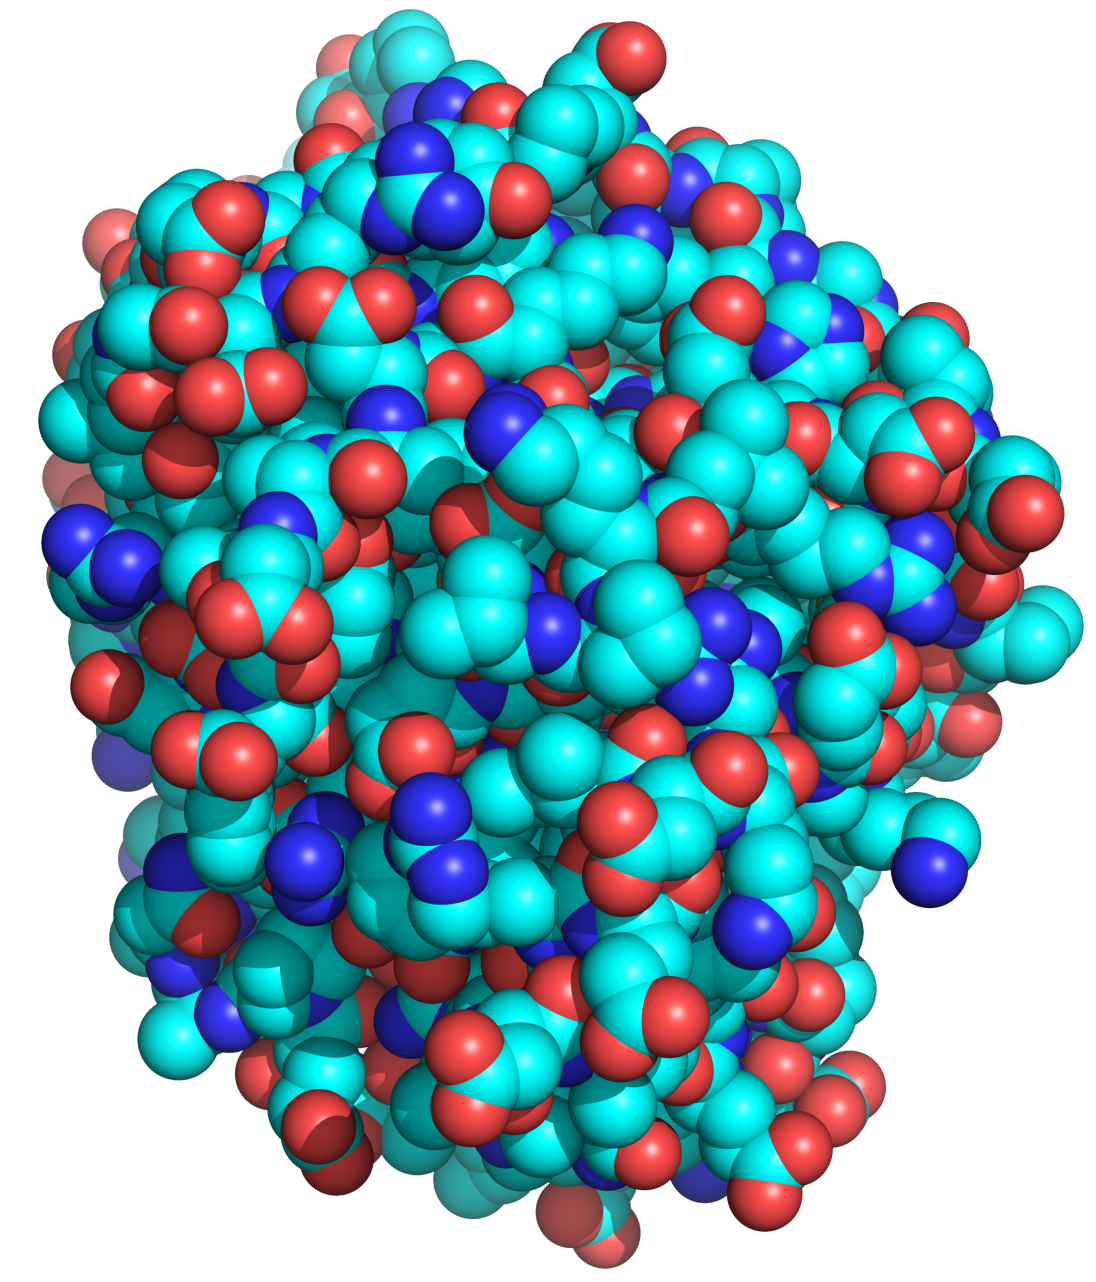
\includegraphics[width=0.15\textwidth]{fig/motiv1} &
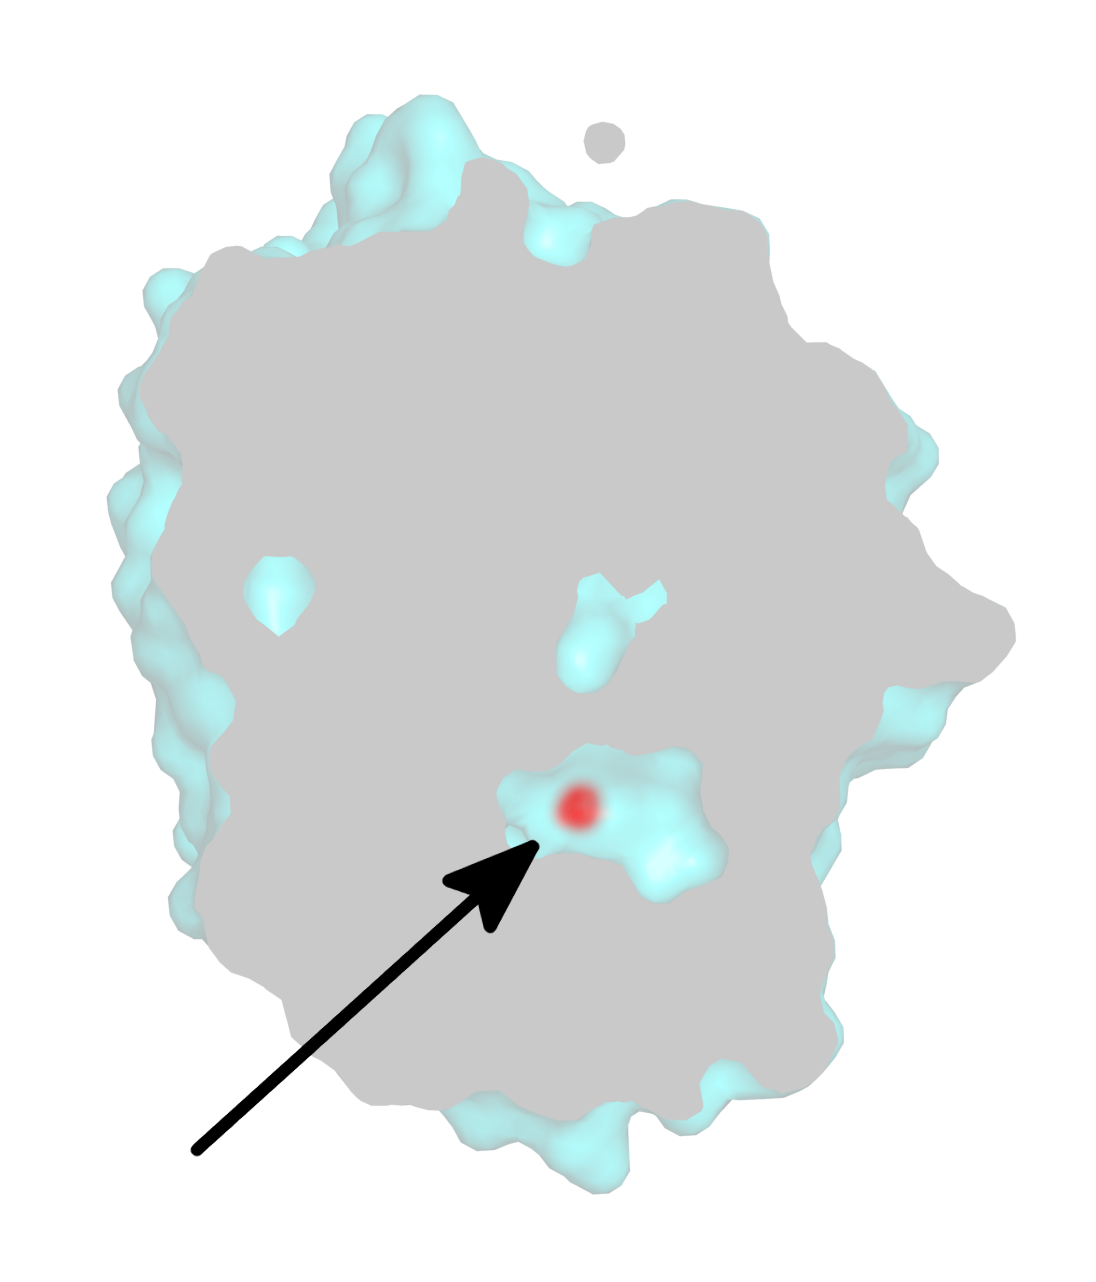
\includegraphics[width=0.17\textwidth]{fig/motiv2lab} &
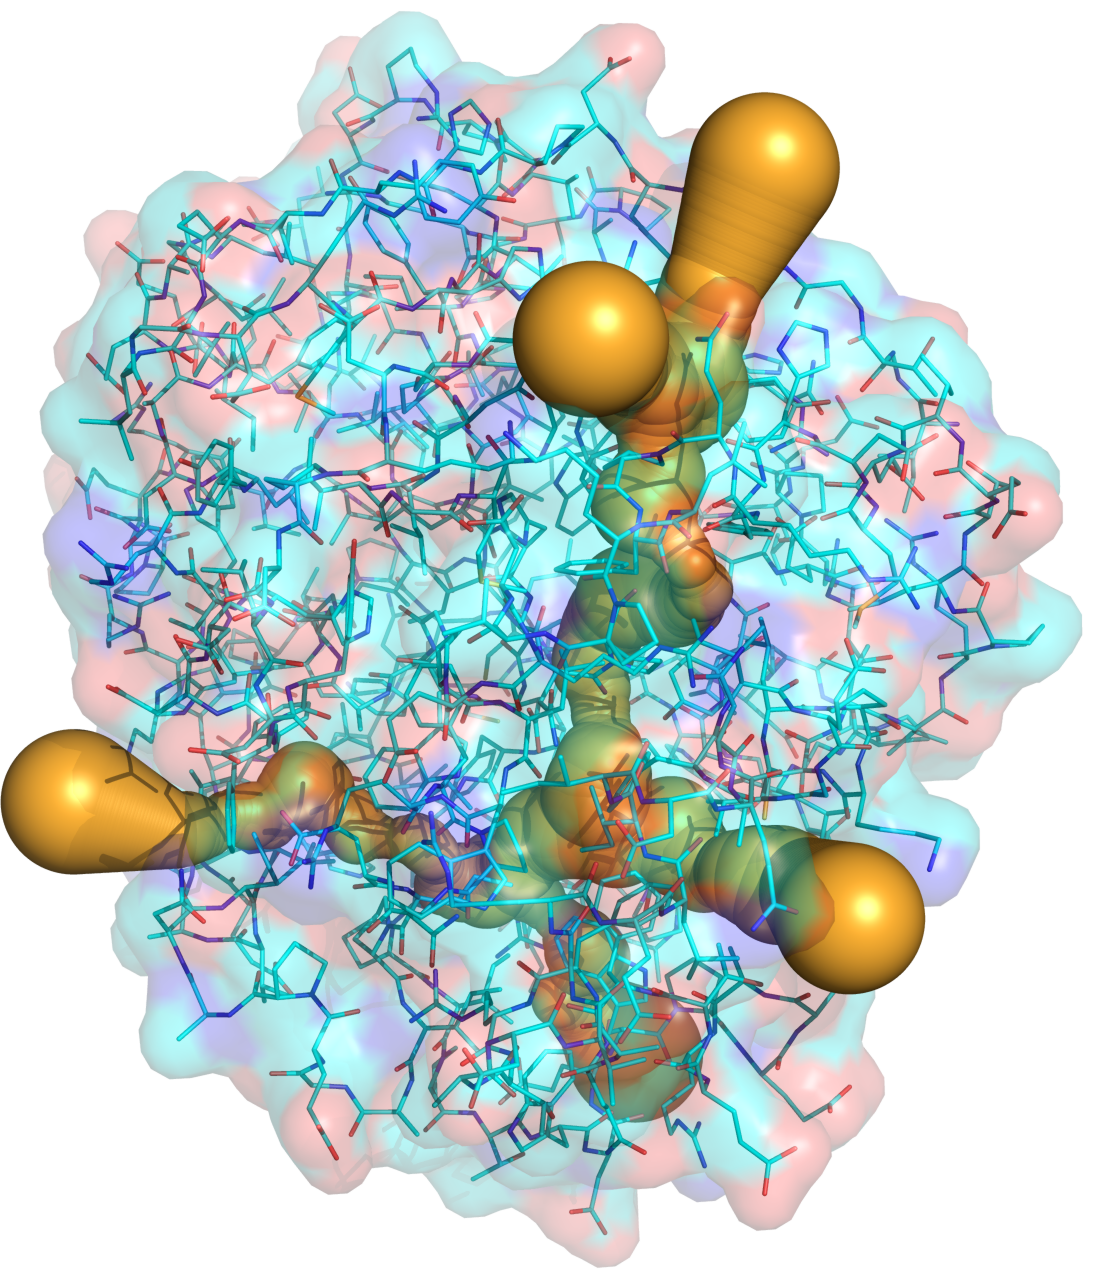
\includegraphics[width=0.16\textwidth]{fig/motiv3} &
\hbox{
\vbox{
\hbox{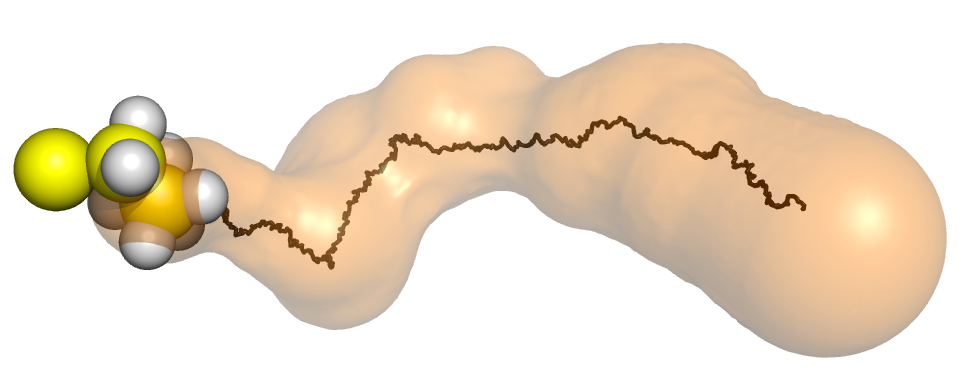
\includegraphics[width=0.25\textwidth]{fig/ta-1} }
\hbox{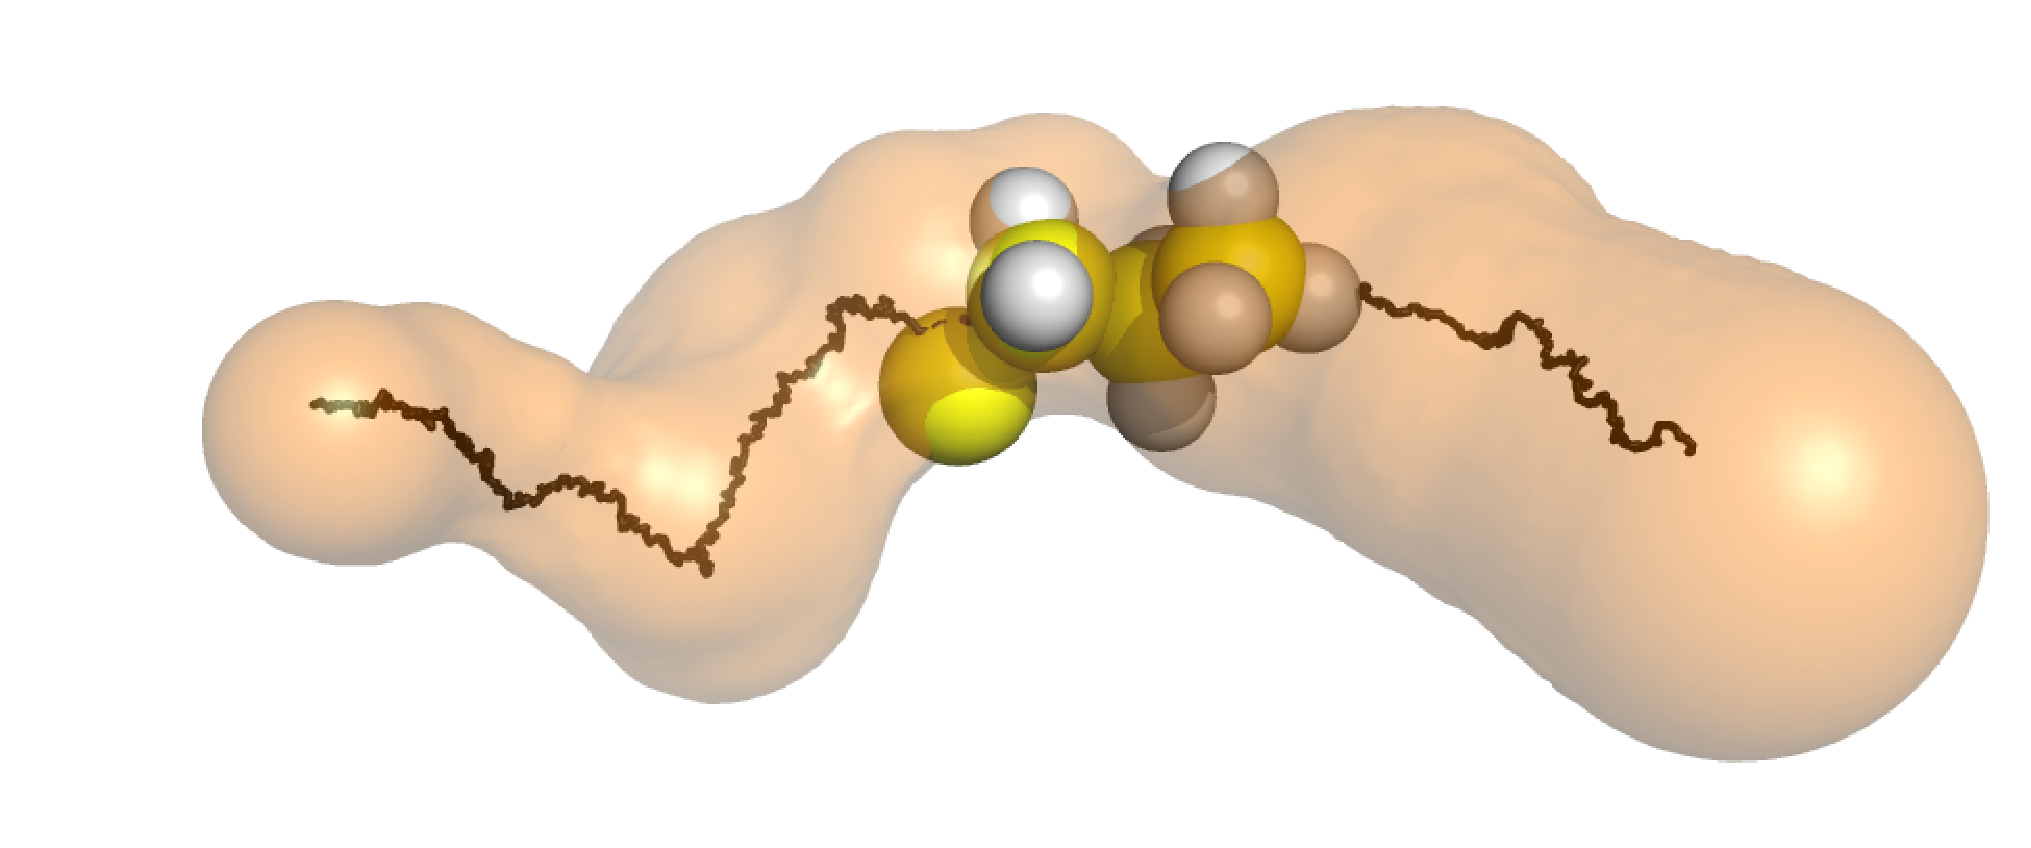
\includegraphics[width=0.25\textwidth]{fig/ta-433}}
} 
}
\\
Protein 1CQW & Active site & Detected tunnels & Example of a  \\
             &            & (orange)          & trajectory
\end{tabular}
}
\caption{\label{fig::motiv}
    Example of tunnel detection in haloalkane dehalogenase.
}
\end{figure}




\red{this is fast copy and paste from previous paper, please rewrite, cut to at ca. 1 page}

%Protein structures are essential components of all living organisms.
Proper understanding of structure and function of proteins is important in many fields, including drug design, agriculture, cosmetics, etc.
%Although this knowledge is still very hard to reveal, several protein structures have been already investigated in sufficient detail. 
Computational methods are often used to analyze the geometry of protein structure,  its shape, surface area, and inner void space. 
Proteins interact with other molecules (small ligands, ribonucleic acid chains, other proteins, etc.) which can lead to changes in properties of the protein or the interacting molecule.
The chemical reaction between the protein and ligand takes places in so called active site, that is accessible 
from the protein surface by a tunnel.

The knowledge about the tunnels is important in many fields..
For example, one task in protein engineering is to change selected properties of a protein, e.g. its stability under different outer conditions~\cite{Koudelakova2013} or activity of the protein towards the other molecules~\cite{Pavlova2009}.
This can be achieved by detecting and studying so called tunnels in proteins which can serve as the transportation paths for the 
ligand from the outside environment to the active site or vice versa. 

The widely used tools for tunnel detection are based on Voronoi diagrams~\cite{yaffe2008,caver3} or 
a 3D grid~\cite{sehnal2013mole,petrek2006caver}.
These methods compute the tunnels assuming a spherical ligand (probe), and the resulting tunnels are represented as a sequence of spheres.
Bio-chemists then decide if such a tunnel can be used to transport a given ligand mainly based on the tunnel lengths and bottleneck (i.e.,
        the radius of the smallest sphere that can traverse the whole tunnel).
%The active sites are usually connected with the protein surface with multiple pathways.
%However, not all paths are biochemically relevant, so only paths with a given minimal bottleneck have to be reported (the bottleneck is
%the radius of the smallest sphere that can traverse the whole tunnel).

%Such decision is however not precise and it requires previous expertise in the domain.
Typical ligands are however non-spherical and therefore it is difficult to estimate their traversability in tunnels
computed for a spherical probe.
It is therefore necessary to consider also the shape of the ligand and possibly also its flexibility.
Due to the increase degrees of freedom (DOF) that need to be considered, the classical Voronoi-based methods cannot be used 
to compute trajectories of the ligands.

\red{TODO}
something about screening: what is it, what's is the input and output, in which applications (research/industry) it is useful.

In this paper, we propose a novel method for computing the trajectories of the flexible ligands in a tunnel represented by spheres.
The proposed work is based on the sampling-based Rapidly Exploring Random Tree (RRT)~\cite{lavalleRRT} planner, which
can cope with many-DOF objects of arbitrary geometry.
The random samples for RRT are generated using the spheres of the tunnel.
To make the transportation easier, a scaled-down version of the ligand is used, similarly e.g. to~\cite{cortes2005path}.
The flexibility of the ligand is modeled using a predefined set of typical conformations.
We propose novel visualization techniques for presenting the results to bio-chemists.
The proposed method can be seen as an extension for the classic tunnel detection tools.

%Recently, researchers started to focus on molecular dynamics simulations and study the behavior of individual tunnels over time~\cite{yaffe2008,caver3,sehnal2013mole}.
%Recently, researchers started to focus on molecular dynamics simulations and studying the behavior of individual 
%tunnels over time~\cite{yaffe2008,caver3,sehnal2013mole}.
%Molecular dynamics is represented as a sequence of frames (molecule snapshots), and the tunnels need to be detected through these frames.
%With the increasing size of simulations the correctness of predicting the most biochemically relevant tunnel increases as well.
%Existing solutions based exclusively on Voronoi diagrams and clustering methods are time and memory consuming
%which also gives the limitation for the maximum number of frames which they are able to analyze.
%In such cases, the biochemists have to select a subset of the whole simulation and perform the analysis only for this selection.
%Such analysis however provides only a rough idea of the tunnel behavior, as important parts of the simulation can be easily omitted.
%This opens new possibilities for alternative solutions enabling to explore the tunnels in each frame of the molecular dynamics.
%In such cases the biochemists have to skip each n-th snapshot or select a subset of the whole simulation and perform the analysis only for this selection.
%The properties of tunnels like bottleneck radius, their length and the surrounding residues can be used
%to estimate suitability of the tunnel for a ligand.
%However, such estimation still involve lot of experience.


\section{Related work}


The analysis of protein structure aiming to reveal the tunnels has been supported by different computational software tools which take the geometry of the protein as an input and explore the inner void space (e.g., CAVER 1.0~\cite{petrek2006caver} or MOLE~\cite{Petrek20071357}). 
Early methods for tunnel detection utilized a discretized 3D grid, where each cell is considered as occupied or free depending
on the presence of atoms of the protein.
Tunnels can be then searched using standard graph-search methods like Dijkstra's algorithm.
Besides, the grid can be used to identify other relevant properties like 
pockets, cavities, or channels~\cite{sehnal2013mole,petrek2006caver}.
%One of the first grid-based approaches to the detection of tunnels in protein is the CAVER 1.0 algorithm by Pet\v{r}ek et al.~\cite{citeulike:6257975}.
The obvious disadvantage of the grid-based methods is the high memory demand and their dependency on the grid resolution.
Due to the high memory consumption, these methods are not suitable for tunnel detection in dynamic proteins and therefore they
are used primarily for analysis of static molecules or individual snapshots of dynamics.

Currently the most widely used approach to tunnel detection is based on Voronoi diagrams (VD) or Weighted Voronoi Diagrams (WVD).
The ordinary VD is computed on points representing centers of all atoms, without considering radii of the atoms.
This may lead to detection of tunnels with incorrect bottlenecks. % i.e., incorrect radius of a smallest probe that can traverse the tunnels.
To consider atoms with different radii, weights of individual points are determined by the van der Walls radii of the atoms in WVD.
An alternative solution is to compute a non-weighted VD on an extended point set, where 
each atom is approximated by several spheres with small radius~\cite{yaffe2008,caver3}.
VD-based methods are memory less demanding, and also faster than the grid-based methods.
The extension of VD-based methods to dynamic molecules requires to construct VD in the frames being analyzed and 
finding correspondences between them.
The existing approaches often use hierarchical clustering to match Voronoi vertices and edges from different frames, which is computationally demanding~\cite{lindow2012dynamic,caverDetails}.

The detected tunnels are evaluated using basic characteristics like bottleneck, length, curvature and a list of surrounding
residues, which are later used to estimate possibility of the interaction.
The biggest disadvantage is that the shape of the ligand is not considered during the tunnel detection and it is therefore
not easy to estimate if (and how) a ligand might traverse the tunnel.

The task of trajectory computation for the non-spherical ligand can be formulated as a path search 
in the related configuration space $\C$.
The dimension of the configuration space is given my the DOF of the ligand, i.e., 6D for a rigid and 6D + $n$ for a flexible
ligand with $n$ DOFs.
%We propose to employ motion planning technique to determine possible trjaectories for a given ligand in the detected tunnels.
%This can be solved by search a high-dimensional configuration space $\C$. % as both 3D translation, rotation possibly with additional DOFs caused
%by the ligand's flexiblity need to be considered.
%The dimension of the configuration space $\C$ is given by the degrees of freedom (6D for a solid ligand and 6D+$n$ for a flexible ligand with
%$n$ rotational bonds).
%The feasible configurations, where the ligand (robot) does not touch and obstacle, form the free region $\CF$.
%The tunnel traversability can be then formulated as a path planning from the start configuration $\qinit \in \CF$ 
%to a goal configuration $\qgoal\in\CF$, where both $\qinit$ and $\qgoal$ are located at the beginning and the end of the
%tunnel, respectively.
%Sampling-based methods like PRM~\cite{kavrakiPRM} or RRT~\cite{lavalleRRT} can be used to search such a path.
The idea of sampling-based motion planning is to randomly sample the configuration space.
The random samples are classified as free or non-free using collision detection and  the free ones are stored into a roadmap.
A path in the roadmap then represents a motion in the workspace.
Beyond robotics, sampling-based motion planners have been successfully applied in computational biology in studies
related to 
protein folding~\cite{al2012motion,gipson2012computational,cortes2010simulating,amato2002using,raveh2009rapid,novinskaya2015improving,songPFintro},analysis of loop motions~\cite{cortes2004geometric}, and even for tunnel detection~\cite{vonasek2016application,vonasek2017tunnel}.
%none of the existing work focuses on the trajectory generation in tunnels.

Rapidly Exploring Random Tree (RRT)~\cite{lavalleRRT} is a single-query motion planning method.
RRT incrementally builds a configuration tree $\T$ rooted at the initial configuration.
In each iteration of RRT, a random configuration $\qrand \in \C$ is generated and its nearest node in the tree $\qnear \in \T$ is found.
A new configuration $\qnew$ is constructed on the line connecting $\qnear$ and $\qrand$ in the distance $\varepsilon$.
If $\qnew$ is collision-free, it is added to the tree.
The algorithm terminates if the tree approaches the goal configuration close enough.

%rrt for molecular: \cite{al2012motion}
%survey \cite{gipson2012computational}
%In our previous works, we proposed to employ RRT also for the purp
%Solutions for tunnel detection using sampling-based methods however have not been discussed yet.
%Sampling-based planners have been used in various applications in robotics~\cite{elbanhawi2014sampling} and also  %,latombe1999motion} and also
% to study proteins, e.g. in  
%loop motions~\cite{cortes2004geometric},
%protein folding~\cite{amato2002using,raveh2009rapid,novinskaya2015improving,songPFintro},
%protein folding~\cite{raveh2009rapid,novinskaya2015improving},
%or protein folding combined with ligand diffusion~\cite{cortes2010simulating}.

In this paper, we propose to employ RRT to compute the trajectory for a given ligand in a given tunnel.
To guide the configuration tree through the configuration space, the random samples are generated gradually using the spheres of the tunnels.
As the tunnels are usually computed on protein models without ligands, they are usually very narrow and a ligand can barely traverse them.
It can be assume that both the protein and the ligand adapt to each other and therefore.
To enable the planner find a solution, the radii of the ligand, and possibly also the radii of the protein atoms, are down-scaled
by a given factor.

The most related work to this paper is the MoMa-LigPath~\cite{cortes2005path}, that is based on the ML-RRT method~\cite{cortes2010simulating,cortes2007mlrrt}.
In comparison to our solution, the method~\cite{cortes2005path} aims for find any path leading towards the active site without
possibility to select a tunnel of interest.


\red{comparison to momaligpath~\cite{cortes2005path} + \cite{guieysse2008structure} }

Ligands are small molecules interacting with the protein. 
Due to the interaction, the relative positions of the ligand's atoms can change.
The ligands can be modeled as a multi-link kinematic chain where the torsional angles phi/psi can change in a given range~\cite{songPFpath}.
After the torsional angles are set, 3D position of each atom of the ligand is computed.
By changing the angles, various conformations can be generated.
However, not all conformations are feasible, which has to be checked using potential energy, which is time consuming.


% in cortes2005path:
%In this paper two kinds of large-amplitude motion are treated: protein loop conformational changes (involving pro-
%tein backbone flexibility) and ligand trajectories to deep active sites in proteins (involving ligand and protein side-chain flex-
%ibility). First studies performed using our two-stage approach (geometric search followed by energy refinements) show that,
%    compared to classical molecular modeling methods, quite   similar results can be obtained with a performance gain of
% several orders of magnitude. Furthermore, our results also  indicate that the geometric stage can provide highly valuable information to biologists.


%The growth of the configuration tree into some regions of the configuration space can however be slowed down due to the narrow passages.
%A narrow passage is a small region of the configuration space containing part of the solution.
%As the samples are generated from uniform distribution in RRT, probability of placing the samples into the narrow passages is low and therefore,
%   the probability of expanding the tree through a narrow passage is small~\cite{hannaWIS}.
%
%This technique is similar to generation of samples near the medial exist of the environment
%medial axis~\cite{wilmarthMAPRM,foskey01hybrid,guibas1999probabilistic,hoff2000interactive,yang2004adapting,amatoOBRRT}.
%or by guiding the growth of the tree around a general path in the workspace~\cite{vonasek2009rrt,denny2014marrt}.


By reducing the scale of the ligand's atomic radii, the configuration tree can explore more areas of the configuration space.
Such techniques has been used for motion planning of deformable objects, 
e.g.,~\cite{frank2008efficient,bayazit2001ligand,alterovitz2008motion,lamiraux2001flexible,kavraki1998towards,gayle2005path} 
and for motion planning of rigid objects in among 
flexible obstacles~\cite{rodriguez2006planning,frank2008efficient,phillips2014representation}.


\section{Preliminaries}

Proteins and ligands are represented by the hard sphere model, where the radius of each sphere (atom) is given by its van der Waals radius.
%Let $\SS \subset \mathbf{R}^3$ denote the union of all spheres, i.e., the geometry of the protein.
%We further assume that a subset of atoms located at the surface, are known. These atoms, reffered to as {\sl surface atoms} in this paper,
%   can be detected as atoms located at $\alpha$-shape of the molecule.
%The tunnels need to be found for a spherical probe $\Sprobe$ of radius $\probe$.
The flexiblity of a ligand is modeled using the set $\L$ of its conformations.
The conformations can be prepared e.g., considering the potential energy using tools like Rosetta.
We assume that a conformation $l \in \L$ can be switched to all other conformations in $\L$.

%Another approach is to model the ligand flexibility using a predefined set of feasible conformations $\L$
%To decrease the computational burden, a set of feasible conformations $\L$ is prepared, e.g. using Rosseta tool.
%The conformations can be prepared using Molecular Dynamics software such as Rosetta.
%For each conformation $c\in \L$ an energy potential is also calculated.
%Let $\L_i$ denote the set of conformations that 
%The transition matrix $M$ defines the possible changes of conformations, i.e., $M(i,j)=1$ if the conformation $c_i \in C$
%can be switched to the confomration $c_j \in C$.

A protein tunnel is described by a sequence of collision-free spheres $T=( (t_i, r_i) )$, $i=1,\ldots,n$, where $n$ denotes the number of spheres,
$t_i=(x_i,y_i,z_i)$ is their 3D position and $r_i$ denotes the maximum collision-free radius of a sphere centered at $t_i$. 
The tunnels can be found by tunnel detection tools like CAVER 3.0~\cite{caver3}.

%from wiki:
%Multiple static structures experimentally determined for the same protein in different conformations are often used to emulate receptor flexibility.[19] Alternatively rotamer libraries of amino acid side chains that surround the binding cavity may be searched to generate alternate but energetically reasonable protein conformations.[20][21]
% 19 = \cite{totrov2008flexible}
% 20 = \cite{hartmann2009docking}
% 21 = \cite{taylor2003fds} 

%Conformations of the ligand may be generated in the absence of the receptor and subsequently docked[13] 
%or conformations may be generated on-the-fly in the presence of the receptor binding cavity,[14] 
%or with full rotational flexibility of every dihedral angle using fragment based docking.[15] 
%Force field energy evaluation are most often used to select energetically reasonable conformations,[16] but 
%knowledge-based methods have also been used.[17]
%13 = https://link.springer.com/article/10.1007/BF00123666

The proteins are dense structures with narrow tunnels.
Depending on the protein, the tunnel bottlenecks can be even less then $1$~\AA, which is too narrow for ligands with more than 2 atoms.
For the purpose of traversability study, the atomic radii of the ligand are scaled down by a factor $s, 0 < s \le 1$.
A discrete set of scales is used, i.e., $s \in \{\smin, \smin+\sdelta, \ldots, \smax\}$, where 
$\smin$ is the minimal allowed scale, $\smax=1$ is the maximal allowed scale and $\sdelta$ is the minimal difference between two scales.
This scaling technique is used also in other tools like MoMaLigPath~\cite{cortes2005path}.

A configuration of the pseudoflexible ligand $q=(x,y,z,r_x,r_y,r_z,l,s)$  is described
by the 3D position $(x,y,z)$ of the reference point of the ligand (e.g., it's geometric center), rotation around $x$, $y$ and $z$ axes,
index of the conformation $l\in \L$ and the actual scale $s$.
All possible configurations form the configuration space $\C$. 
A configuration is collision-free if there is no intersection between the protein atoms and ligand atoms scaled by $s$.
%The set of all feasible configurations at scale $s$ is denoted $\CFD \subseteq \C$.


\section{Ligand traversability}

The task of the traversability study is to determine if a given ligand can traverse  a given tunnel in the protein.
We propose a RRT-based method to compute the trajectories of the ligand.
As the tunnels are usually computed on proteins without ligands, their are usually very narrow and the classic RRT would
suffer from the well known narrow passage problem~\cite{hannaWIS}.

To cope with the narrow passage problem, the random samples are not generating from the whole configuration space.
Instead, they are generated using the spheres of the tunnel.
The main loop of the method is described in Alg.~\ref{alg::main}.
In each iteration, a random sample $\qrand$ is generated, its nearest node $\qnear\in\T$ in the tree is found.
The nearest-neighbor search between the $\qrand$ and the tree is realized using the weighted 6D Euclidean metric considering
both 3D rotation and 3D translation.

To guide thee growth of the tree through the tunnel, a moving virtual goal is used~\cite{vonasek2009rrt}.
The virtual goal $v$ is the index of a sphere, around which the random samples are generated with probability $\gb$.
%The random samples are not generated only from whole $\C$, as in the original RRT, but the sampling
%is guided using moving virtual goal~\cite{vonasek2009rrt}.
After the tree reaches the sphere $t_v \in T$, i.e., the distance of the tree to the center of $t_v$ is
less than a predefined threshold $\dt$, the virtual goal is moved to successor of the last sphere in the tunnel
that is reached by the tree (lines~\ref{alg::main:a}--\ref{alg::main:b} in Alg.~\ref{alg::main}).
Setting the virtual goal to this successor allows the tree to ``skip'' such parts of the tunnels that are
not traversible or reachable by the ligand.
The algorithm terminates after the predefined number of planning trials $\Imax$ or if the tree reaches
the last sphere in the tunnel, i.e., when $v = N$.

The random samples $\qrand$ are generated around the virtual goal.
The translation of $\qrand$ is generated from Normal distribution centered at $t_v$ with radius $R_v$.
The radius $R_v$ is set as the absolut distance from the tunnel centerline, e.g. $R_v=3\AA$.
Alternatively, $R_v$ can be set to $R_v=r_v$ according the radius of the tunnel at the virtual goal.

\linesnumbered
\begin{algorithm}[h]
%\setstretch{\straa}
\caption{\label{alg::main}main loop of the RRT planner}
\KwIn{
    tunnel $T=(t_i, r_i), n=1,\ldots,N$ represented by $N$ spheres,
    initial configuration $\qinit$,
    goal configuration $\qgoal$,
}
\KwData{
   ligand conformations $\L$,
   scale limits $\smin, \smax$ and $\sdelta$
}
\KwOut{
    configuration tree $\T$\;
}
\hrule
$v = 0$; // index of the virtual goal\\
$iteration = 0$\;
\While{$iteration < \Imax$ {\bf and}  $v < N$}{
    \eIf{$rand() < \gb$}{
        $\qrand$ = random sample around actual virtual goal $t_n \in T$\;
    }{
        $\qrand$ = random sample from $\C$\;
    }
    $\qnear$ = nearest node in $\T$ towards $\qrand$\;

    expand($\qnear$)\;

   % \For{$q \in S$}{
    %    $\T$.addNode($q$)\;
    %    $\T$.addEdge($\qnear, q$)\;
    %}

    \For{$i= N-1,N-2,\ldots,v+1,v$}{ \nllabel{alg::main:a}
        $d$ = nearest node in the tree towards sphere $t_i$\;
        \If{$d < \dt $}{
            $v = i+1$; // new virtual goal found\;
            {\bf  break}\;
        }
    } \nllabel{alg::main:b}
    $iteration = iteration+1$\;
}
\return $\T$\;
\end{algorithm}


The core of the proposed method is the expansion procedure (Alg.~\ref{alg::expand}) which generates new collision-free nodes around $\qnear\in\T$.
For each ligand conformation $l \in \L$, the expansion procedure attempts to find a new collision-free configuration around $\qnear$ with a maximal
scale.
First, the maximal scale $\smax$ is tested and $m$ random samples are generated around $\qrand$ and tested for collision.
The nearest collision-free sample towards $\qrand$ is selected and added to the tree.
If none of the tested samples is collision-free, the scale is reduced to $\smax-\sdelta$ and the searches continues
until a free collision-free samples is found or until the mimimal reduced-scale $\smin$ is reached.

The sampling-based methods are sensitive to the employed metric, especially if the objects are not symmetrical, which is the
case of the non-spherical ligands.
To consider the actual shape of the ligand (which is different in each conformation) and to allow finding such configurations
that approach $\qrand$, the distance between newly generated configurations and $\qrand$ is measured as the smallest
distance between an atom of the ligand placed at $q$ and the 3D position of $\qrand$ ($\da(q,\qrand)$ on line~\ref{alg::expand:a} in
        Alg.~\ref{alg::expand}).

The 3D position of $q$ is generated using Normal distribution $N(0,\sigma^2)$ around $\qnear$, where $\sigma^2$ is the predefined
parameter.
The rotation part of $q$ is generated using $U(0,2\pi)$.
The expansion begins with the largest scale $s$ and if less then $m$ collision-free samples are generated
with $s$, the next lower $s$ is used.
The expansion step is repeated for each conformation $l \in L$.


\begin{algorithm}[h]
%\setstretch{\straa}
\caption{\label{alg::expand}expand}
\KwIn{
   configuration $\qnear$ to be expanded,
   random configuration $\qrand$
}
\KwData{
   ligand conformations $\L$,
   scale limits $\smin, \smax$ and $\sdelta$
}
%\KwOut{
%    set $S$ of collision-free configurations reachable from $\qnear$\;
%}
\hrule
\ForEach{$l \in \L$}{
    \ForEach{$s \in (\smax,\smax-\sdelta, \ldots, \smin)$}{
        $\qnew = \emptyset$; // empty configuration\\
        \For{$i = 1,\ldots,m$}{
            $q=\qnear$\;
            $q.position$ = random 3D position around $\qnear$\;
            $q.rotation$ = random 3D rotation\;
            $q.l = l$\; 
            $q.s = s$\;
            \If{isCollisionFree($q$)}{
                \If{$\qnew = \emptyset$ {\bf or} $\da(q, \qnear) < \da(\qnew,\qnear)$}{ \nllabel{alg::expand:a}
                    $\qnew = q$\;
                }
            } 
        }
        \If{$\qnew \ne \emptyset$} {
            $\T$.addNode($\qnew$)\;
            $\T$.addEdge($\qnear,\qnew$)\;
            {\bf break;} // go to next conformation
        }
    }
}
%\return $S$\;
\end{algorithm}

The configruation tree can be expanded by up to $|\L|$ new configurations, as for each ligand conformation at most
one new configuration can be added.
The most time consuming part of the method is the collision-detection, which is called $m|\L|$ in each expansion step.
The collision detection can be evaluated fast using hiearchical methods like OBB trees, which is implemented e.g. in the OZCollide library~\cite{ozcollide}

\def\tmpa{0.16\textwidth}

\begin{figure}
\centering
\begin{tabular}{cccccc}
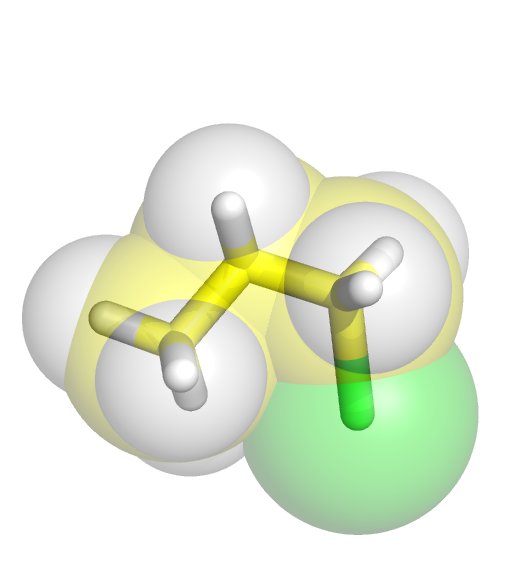
\includegraphics[width=\tmpa]{fig/m003-000} &
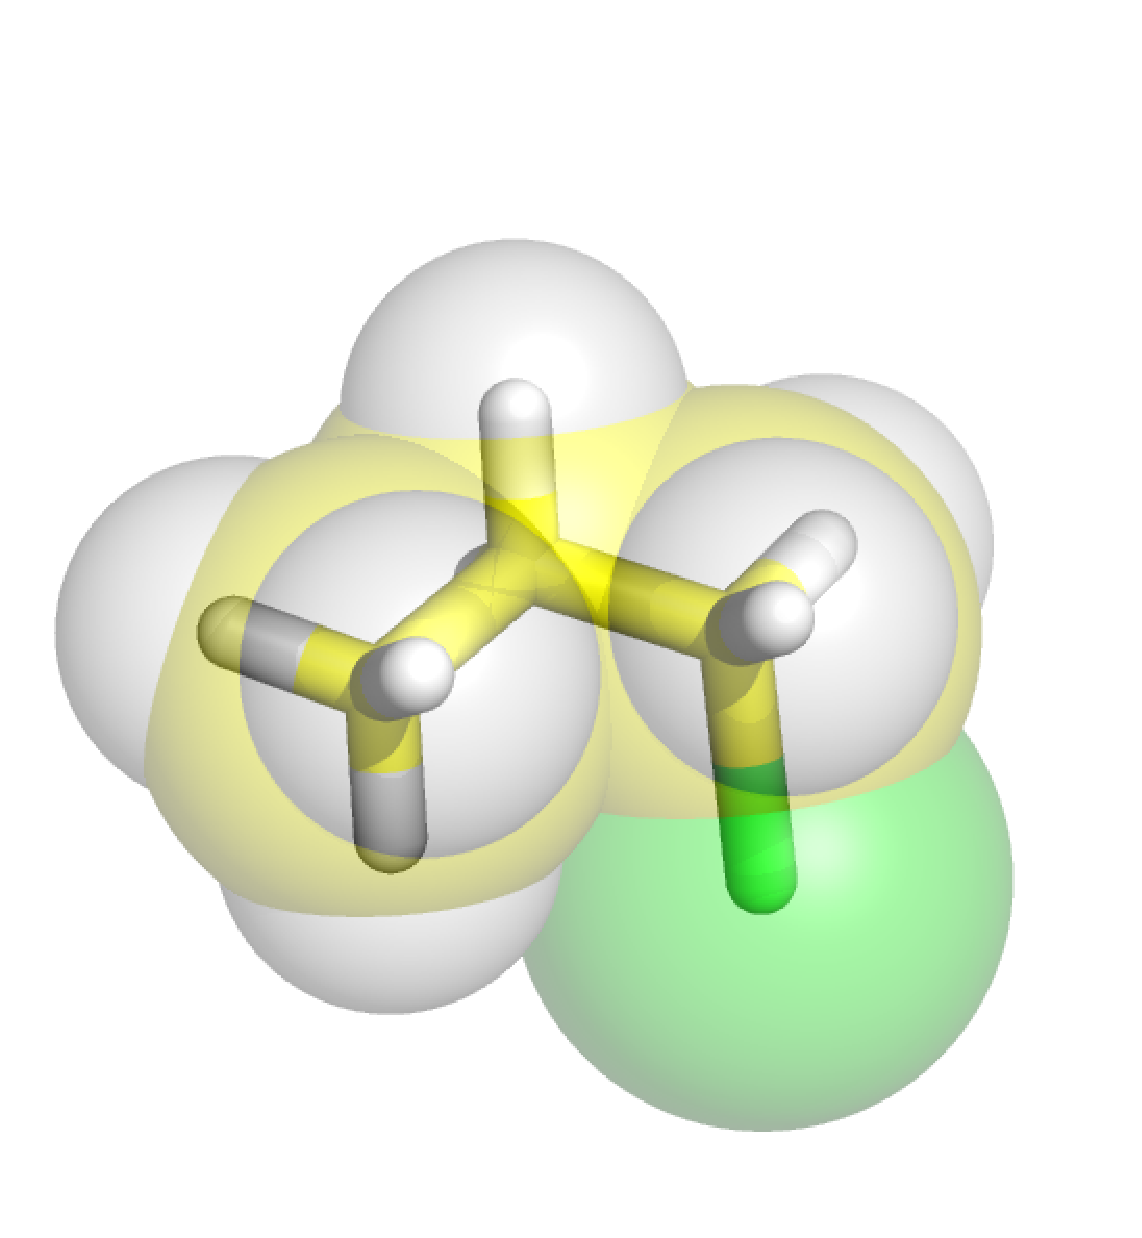
\includegraphics[width=\tmpa]{fig/m003-001} &
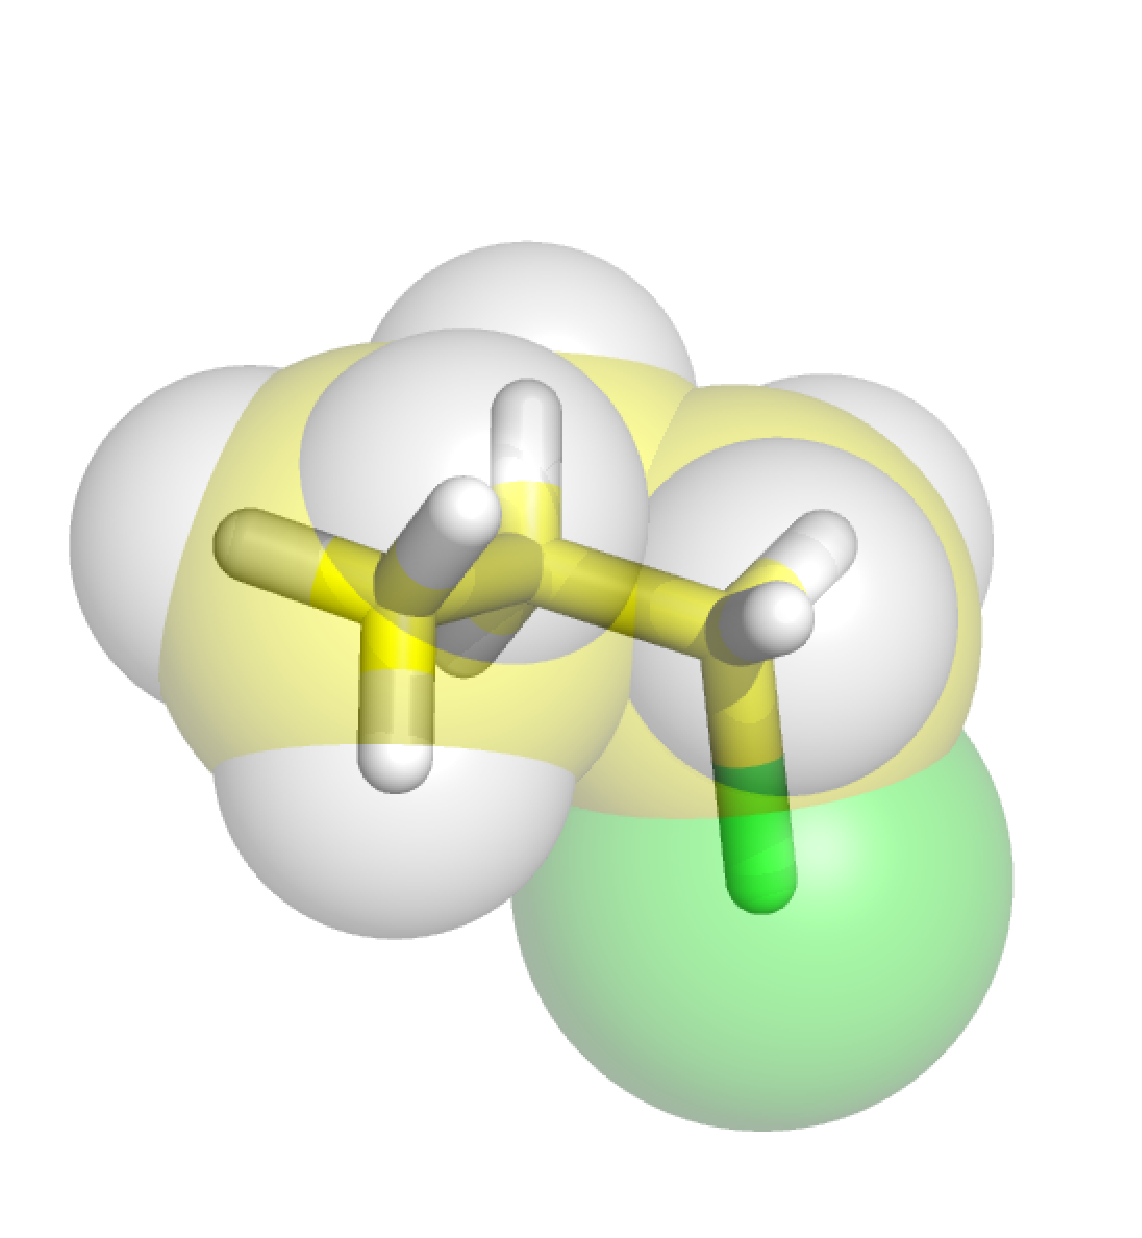
\includegraphics[width=\tmpa]{fig/m003-002} & 
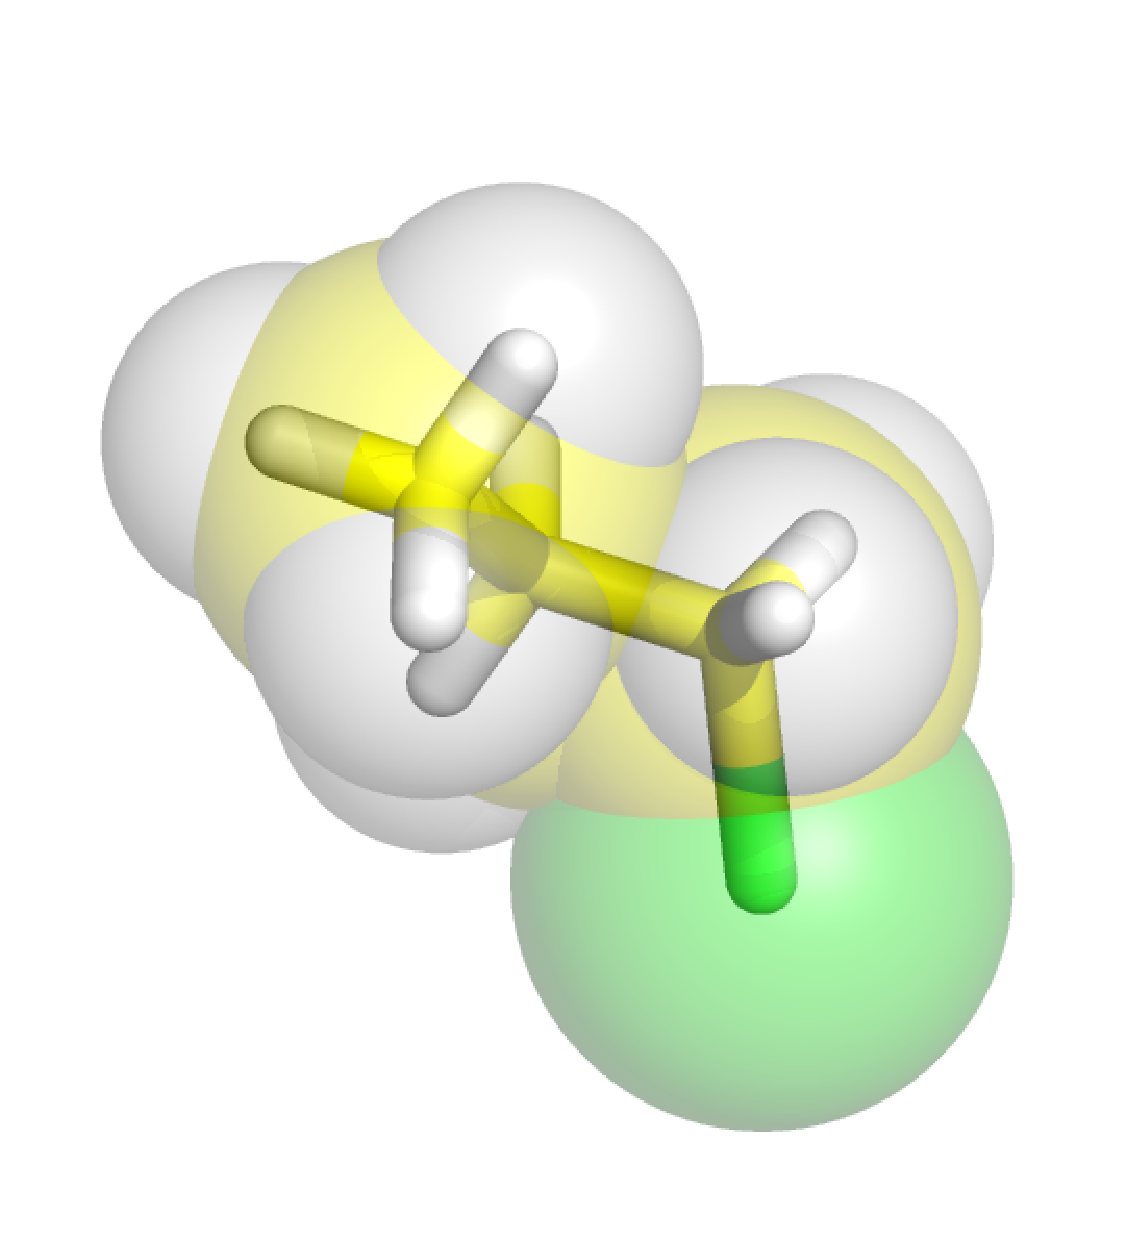
\includegraphics[width=\tmpa]{fig/m003-003} & 
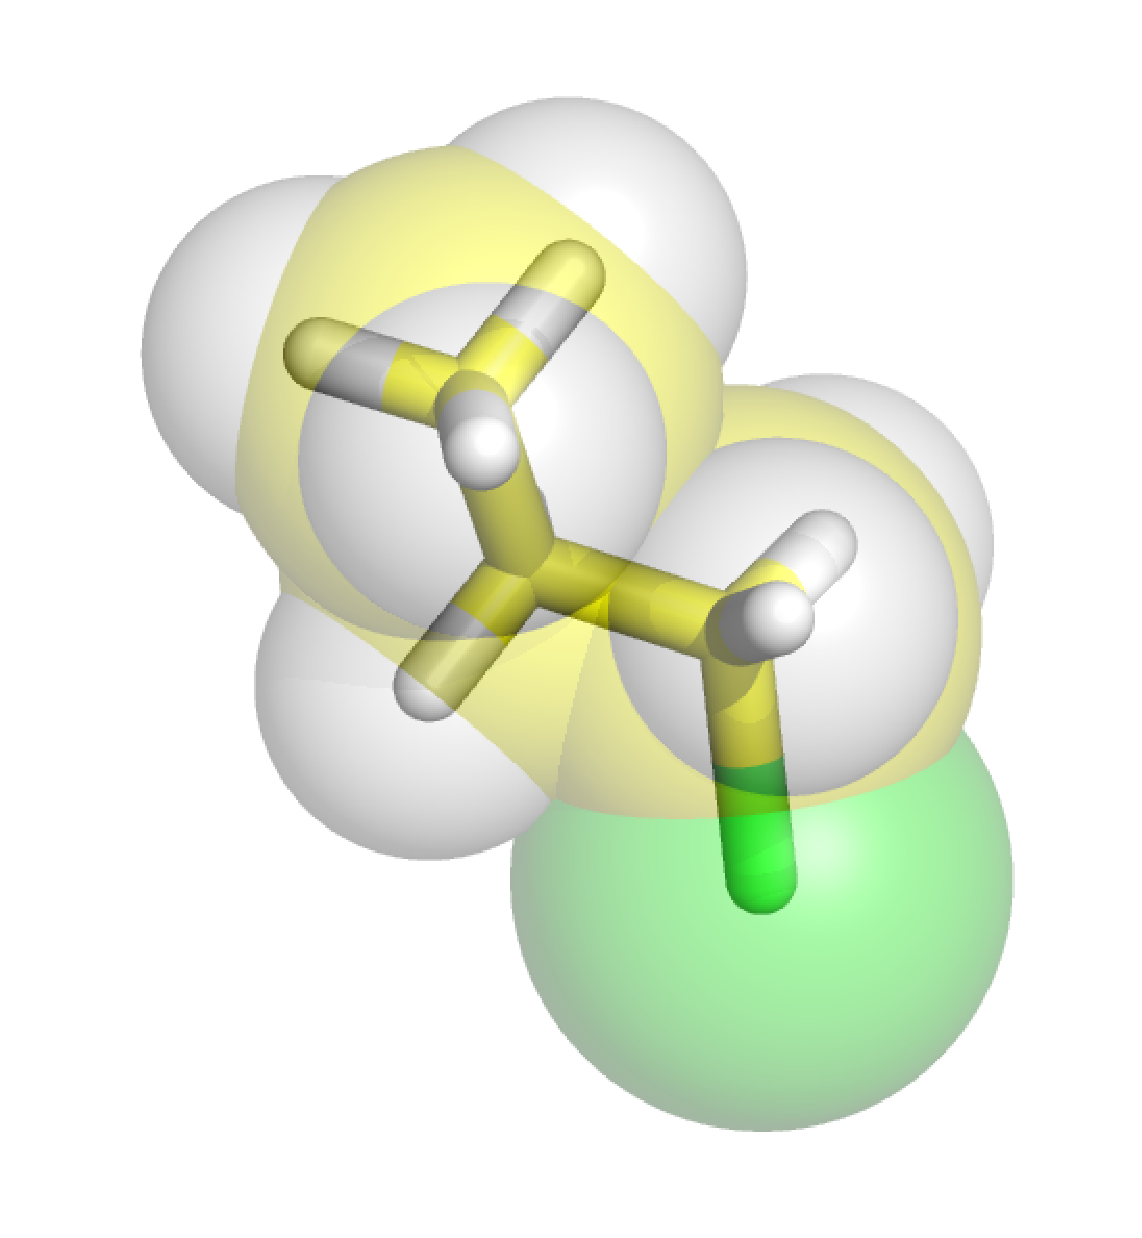
\includegraphics[width=\tmpa]{fig/m003-004} & 
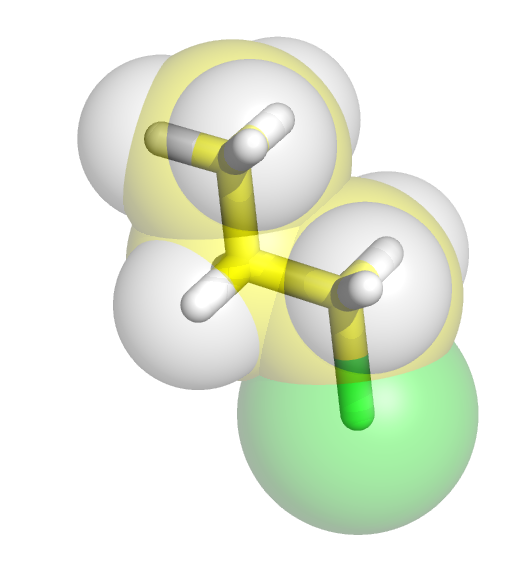
\includegraphics[width=\tmpa]{fig/m003-005} \\
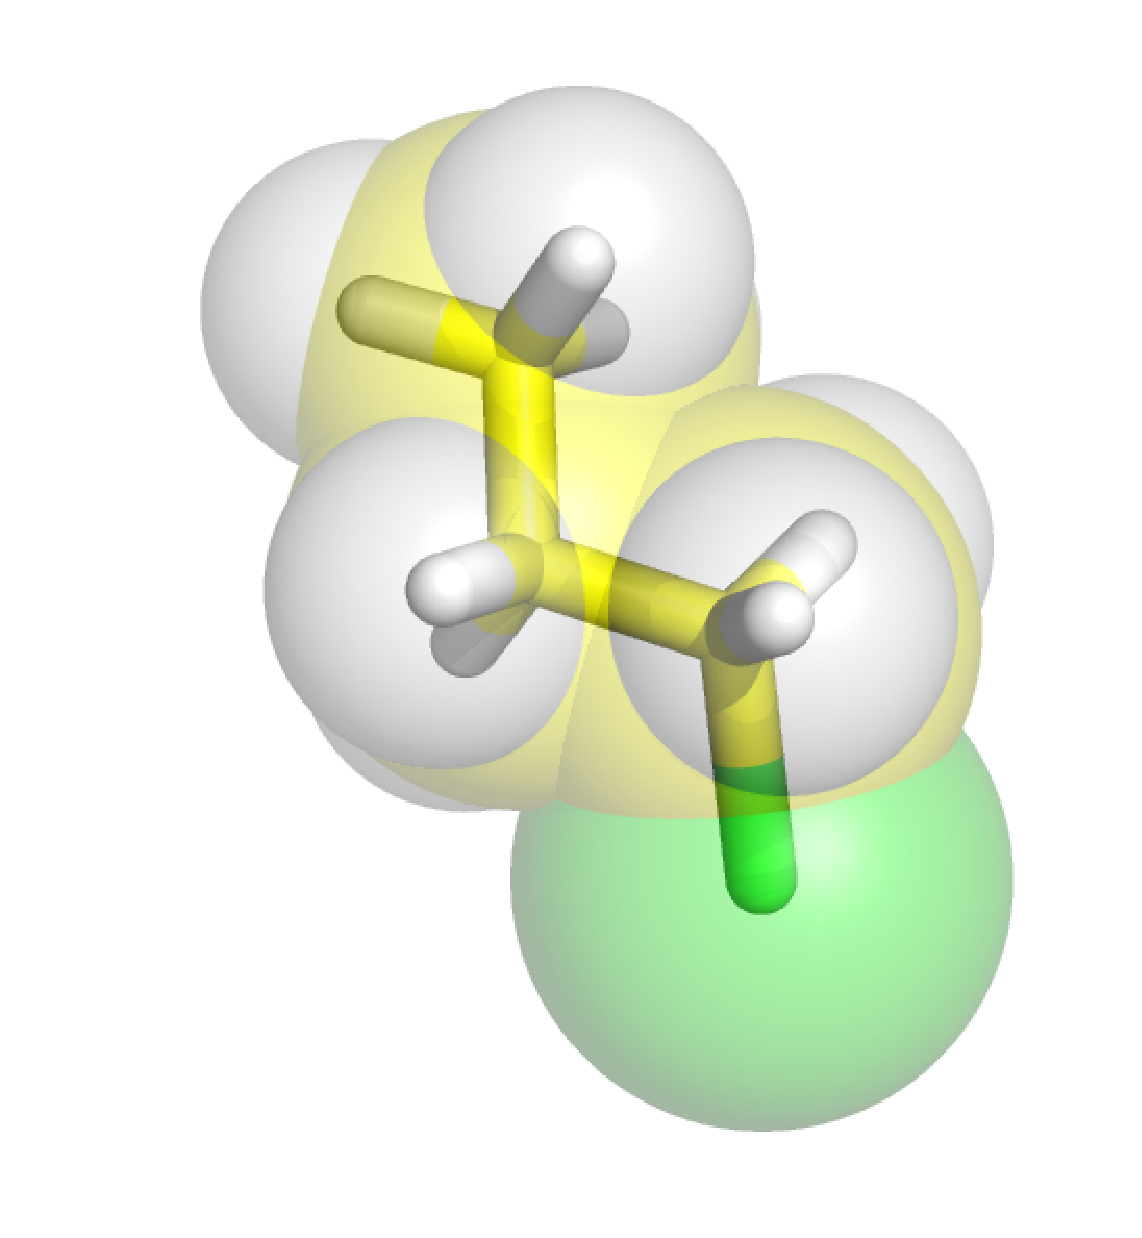
\includegraphics[width=\tmpa]{fig/m003-006} &
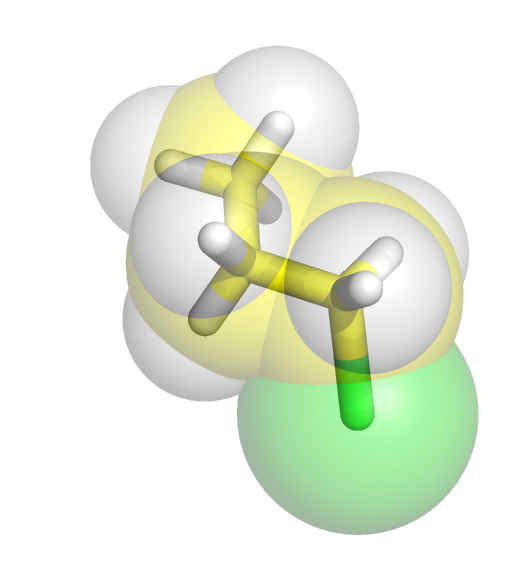
\includegraphics[width=\tmpa]{fig/m003-007} &
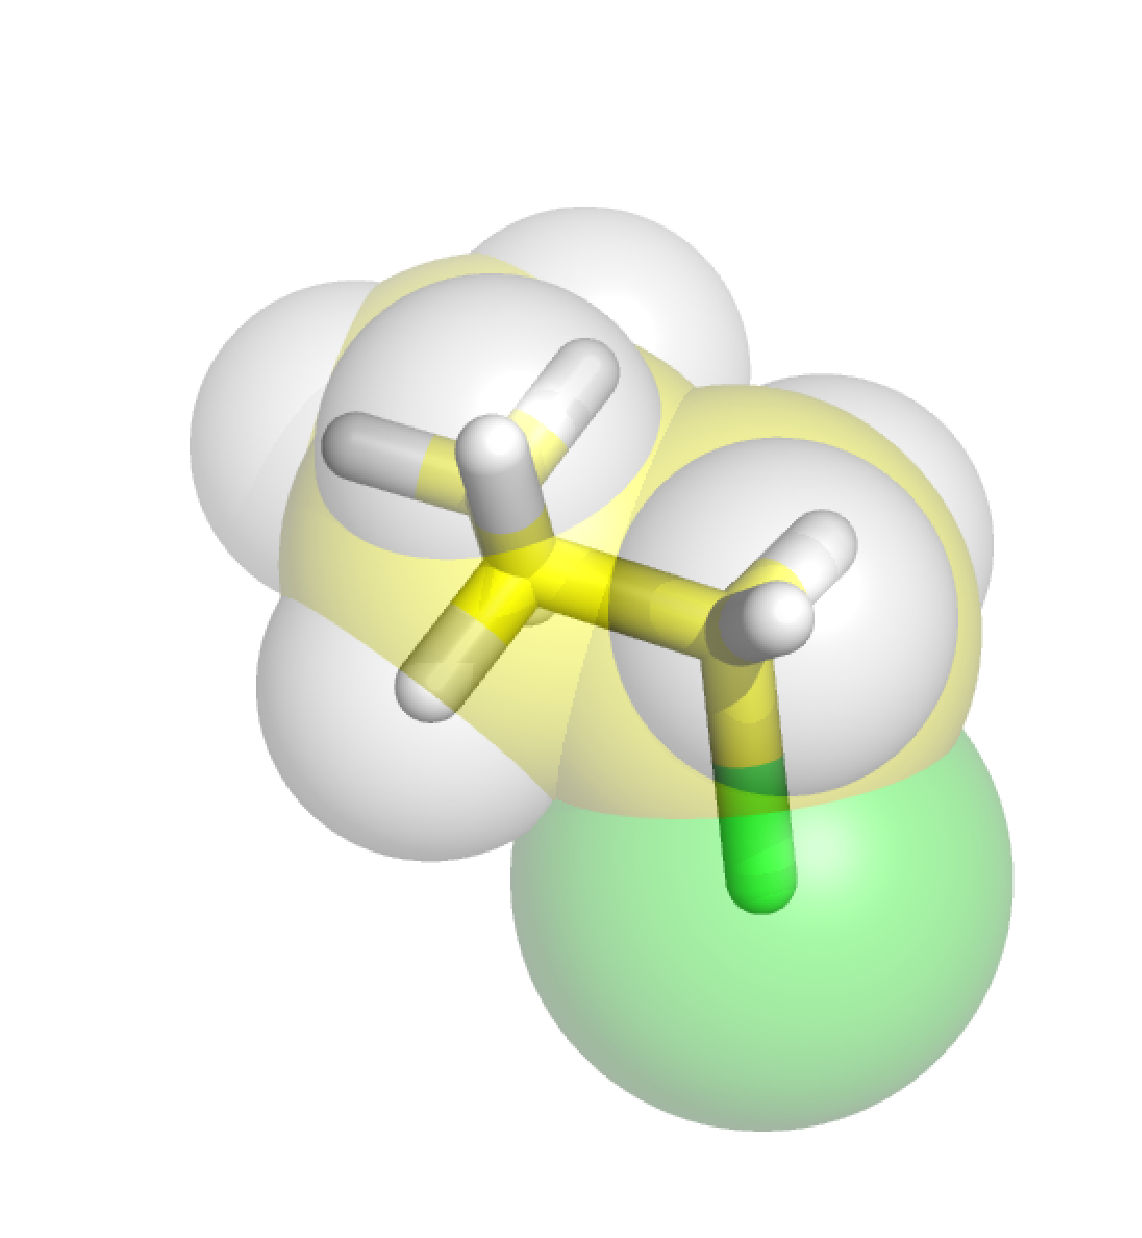
\includegraphics[width=\tmpa]{fig/m003-008} & 
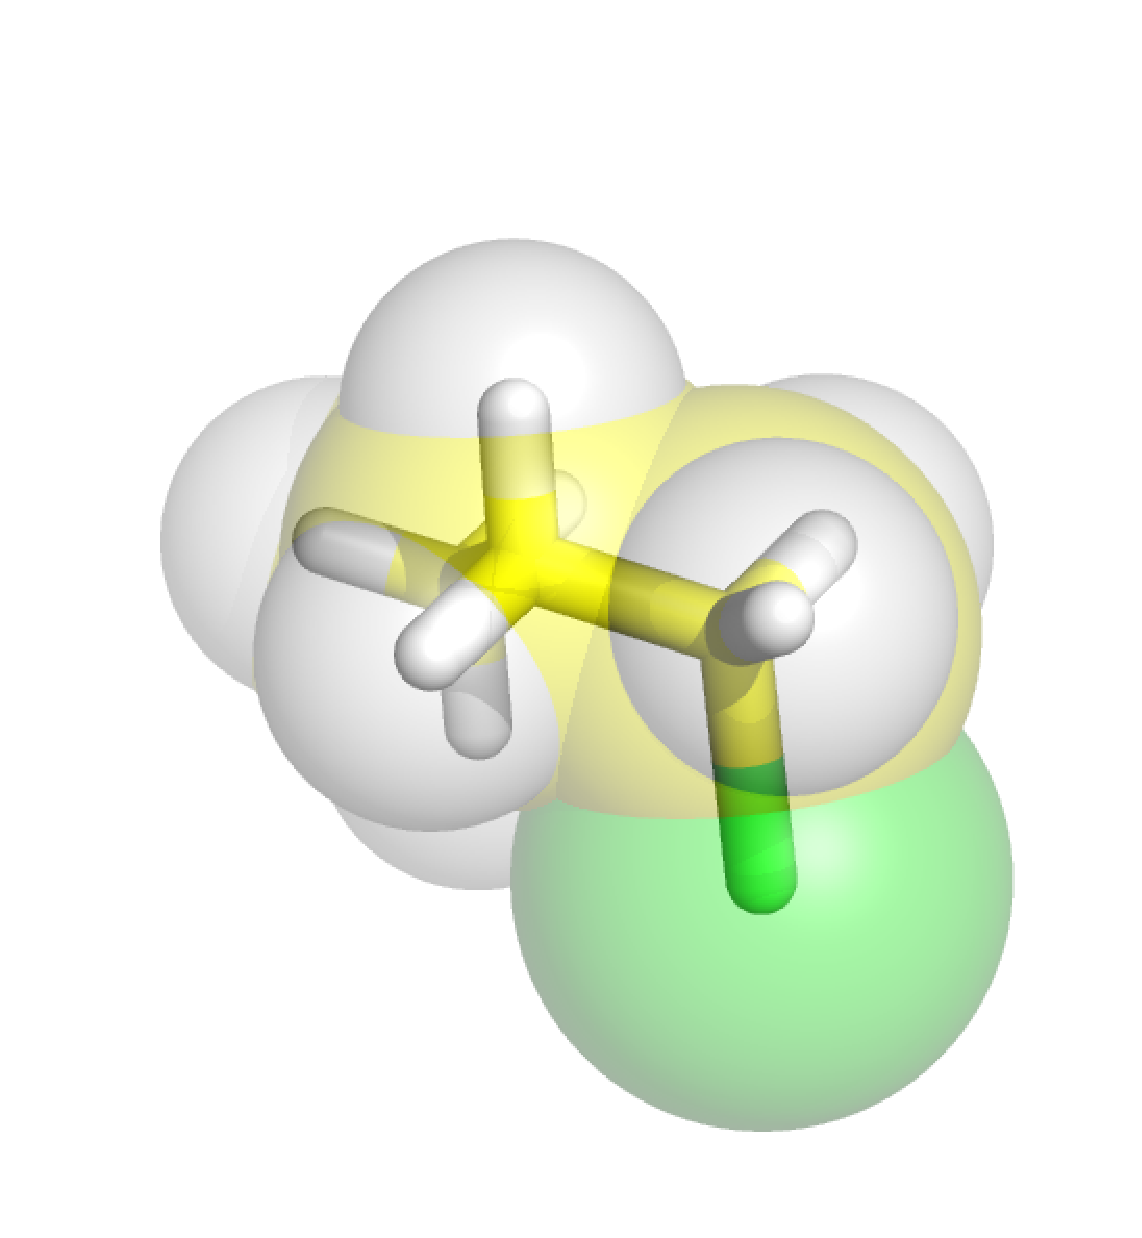
\includegraphics[width=\tmpa]{fig/m003-009} & 
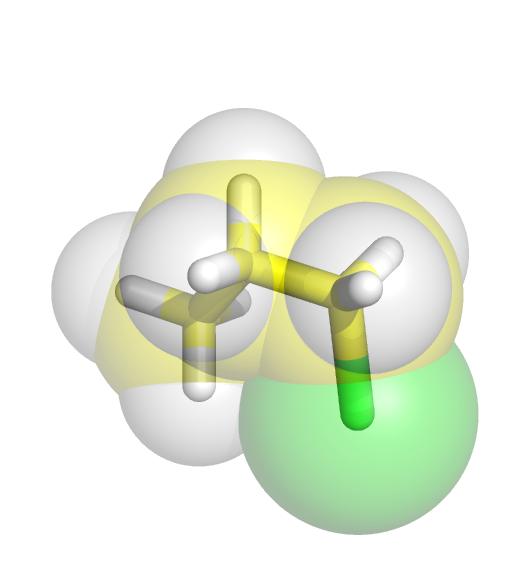
\includegraphics[width=\tmpa]{fig/m003-010} & 
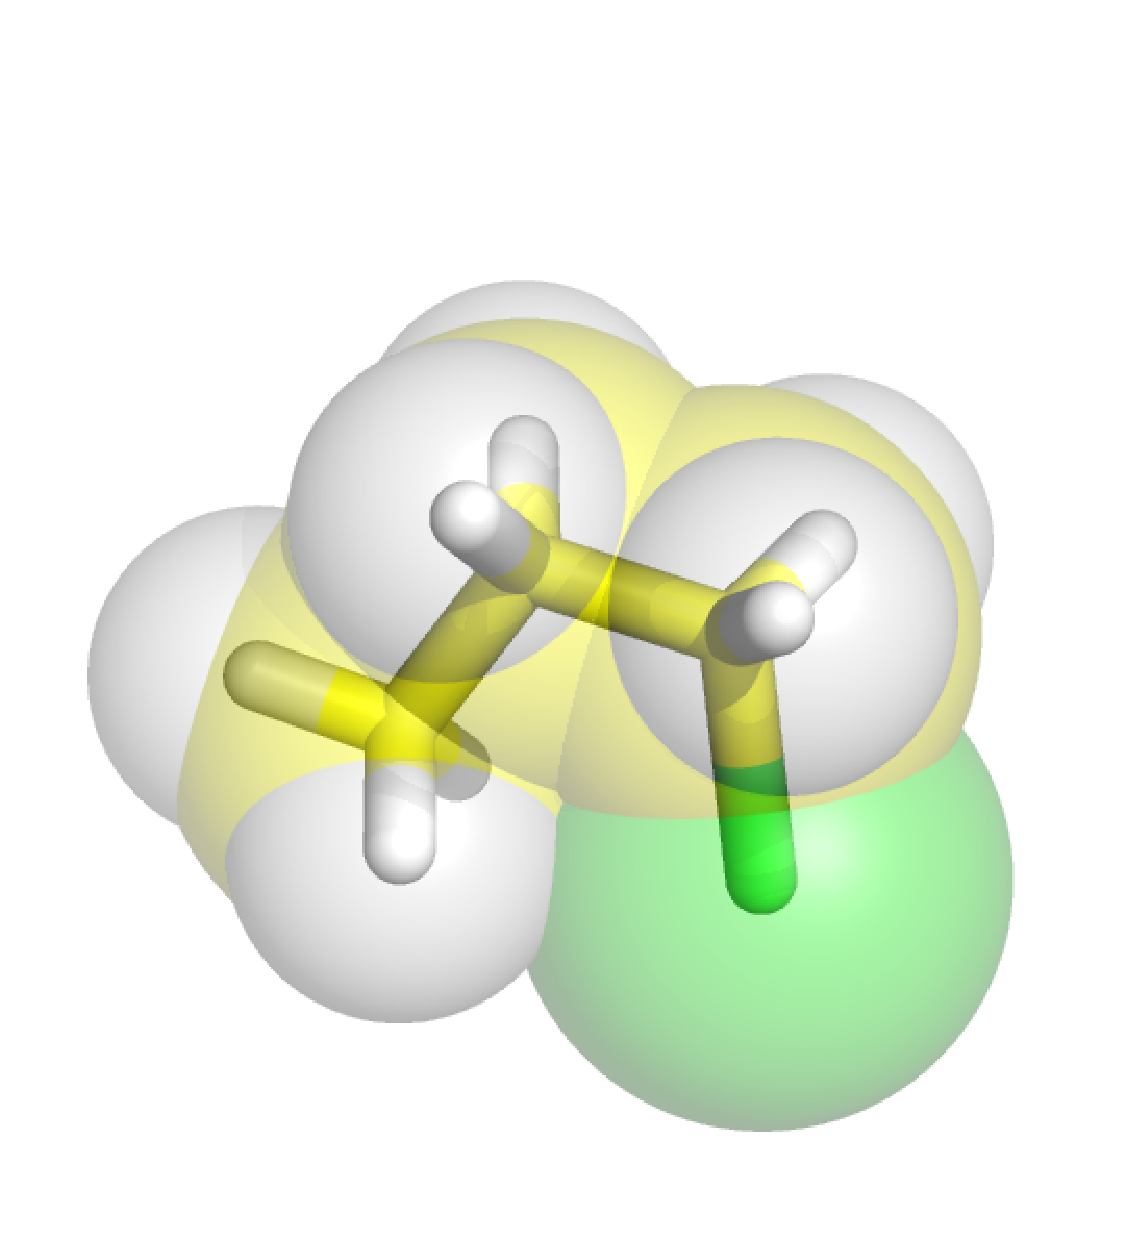
\includegraphics[width=\tmpa]{fig/m003-011} \\

\end{tabular}
\caption{todo and maybe delete}
\end{figure}


\section{Visualization of results}

The result of the proposed planning method is a tree of collision-free configurations, from which a path leading from $\qinit$
to the nearest node towards $\qgoal$ can be found.
Due to stochastic nature of RRT, it is not guaranteed that the tree always reached the goal configuration $\qgoal$.
Despite, a trajectory leading as close as possible towards $\qgoal$ is extracted from the tree.

To present the results to chemicists ...

\red{Adam: }
As described above, our approach enables to estimate the probability that a ligand given a minimum scale passes through a tunnel.
On the other hand, the probability does not describe any details about the ligand's passage, e.g., how hard it is to pass some part of the tunnel, which trajectory is the most used, etc.
Moreover, it is not feasible to directly visualize and explore the resulting trajectories due to the visual clutter (see Fig.~\ref{fig:trajectories} left) caused by their high number and close proximity.
Therefore, we propose to extract and visualize the complex information about the ligand's passage through a tunnel.
In this manner, we aim to further support the decision process of a chemist about a tunnel.
In order to do that, we employ an ensemble of resulting trajectories, and we compute and visualize the following tunnel properties:
\begin{itemize}
  \item \textbf{Accessibility} --- The probability of the ligand that it reaches a tunnel's part.
  \red{ i.e., number of trajectories ending in the tunnel part over all trajectories? }
  \item \textbf{Ligand scale} --- The scale of the ligand wheh it passes a tunnel's part.
  \item \textbf{Throughput} --- The probability of the ligand that it passes through a tunnel's part.
\red{ i.e., the conditional probability we discussed in the mail?}
\end{itemize}
During visualization, we map these properties onto a tunnel's surface (see Fig.~\ref{fig:properties}) so that they can be visually correlated with, e.g., the tunnel's shape.

\begin{figure}
\centering
\begin{tabular}{ccc}
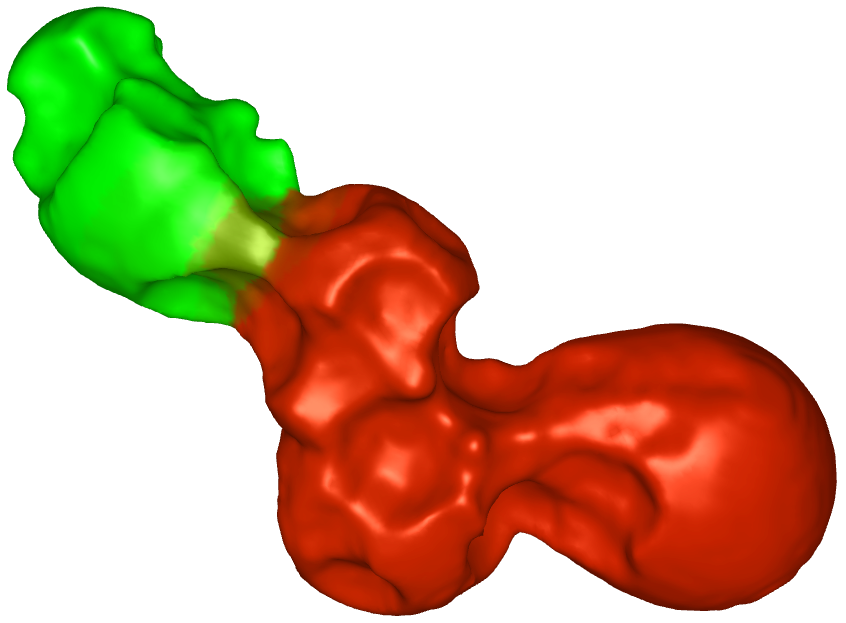
\includegraphics[width=0.3\textwidth]{fig/accessibility}
\quad & \quad
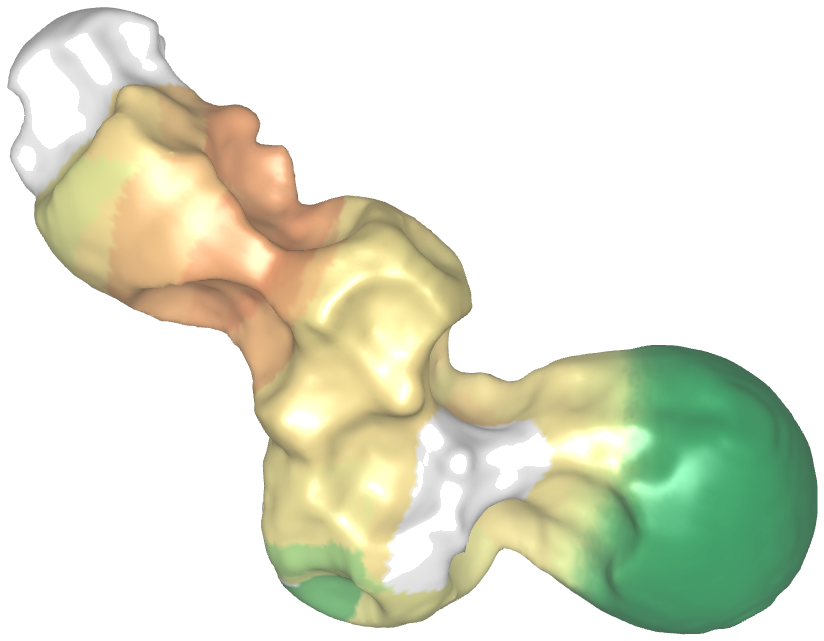
\includegraphics[width=0.3\textwidth]{fig/ligand-scale}
\quad & \quad
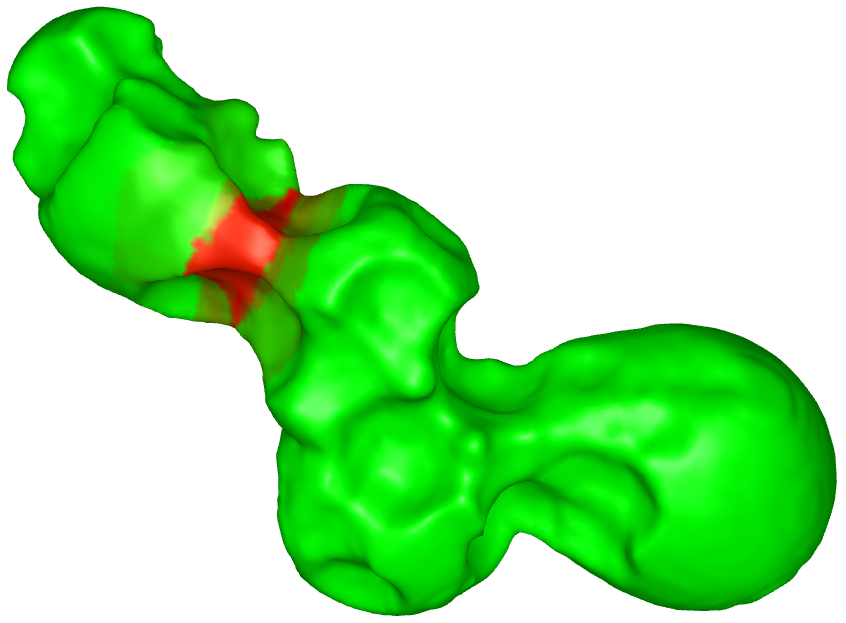
\includegraphics[width=0.3\textwidth]{fig/throughput}
\end{tabular}
\caption{Tunnel properties mapped onto its surface.
Left: Accessibility --- green denotes parts that were accesed by the ligand easily while red denotes parts that were accessible only in about 10\% of computations.
Middle: Ligand scale --- the average scale of the ligand was \~50\% in orange parts, \~60\% in yellow parts, \~80\% in yellow to green parts and \~100\% in green parts.
Right: Throughput --- green denotes parts that are highly probable to be passed by the ligand while red denotes those that were hard to pass.}
\label{fig:properties}
\end{figure}

\red{can you please tell in detail how is the accesibility/liugand/throughput mapped to the tunnel surface/spheres? }

Moreover, we analyze the whole set of trajectories in order to convey the most important trajectories that enabled the ligand to pass or that prevented it from passing.
In order to visualize the important trajectories we first cluster the trajectories according to their similarity. 
\red{can you please add some details how is the similarity counted? Maybe a short description of even equation.}
Then we choose a representant from each cluster a we visualize its trajectory in 3D using a polyline.
\red{please some reference to the hierarchical clustering}.
Moreover, we map the representant's cluster size onto the width of the polyline.
In this manner, we are able to convey the information about all different trajectories together (see Fig.~\ref{fig:trajectories} right).

\begin{figure}
\centering
\begin{tabular}{cc}
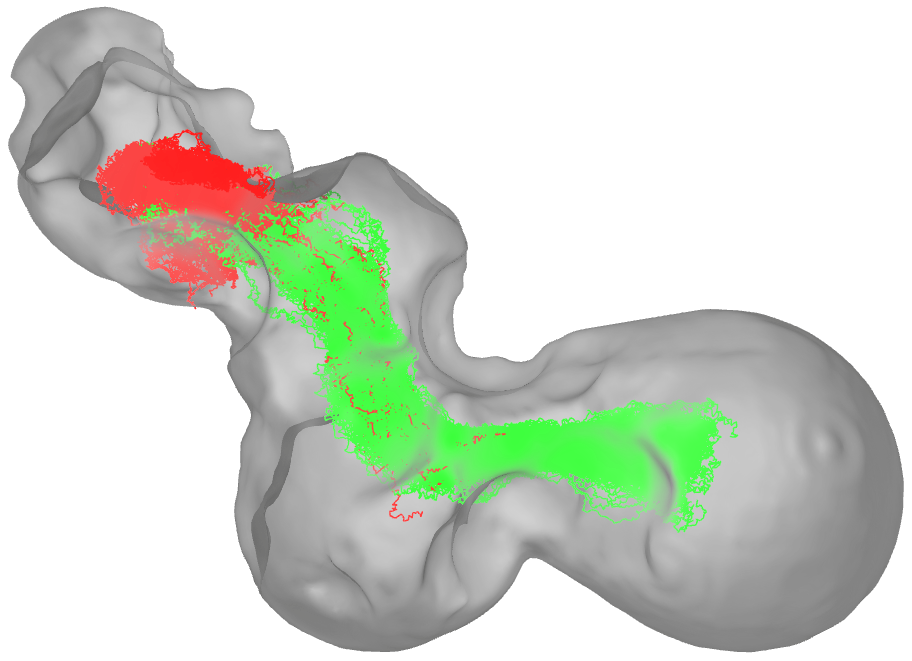
\includegraphics[width=0.45\textwidth]{fig/trajectories-all}
\qquad & \qquad
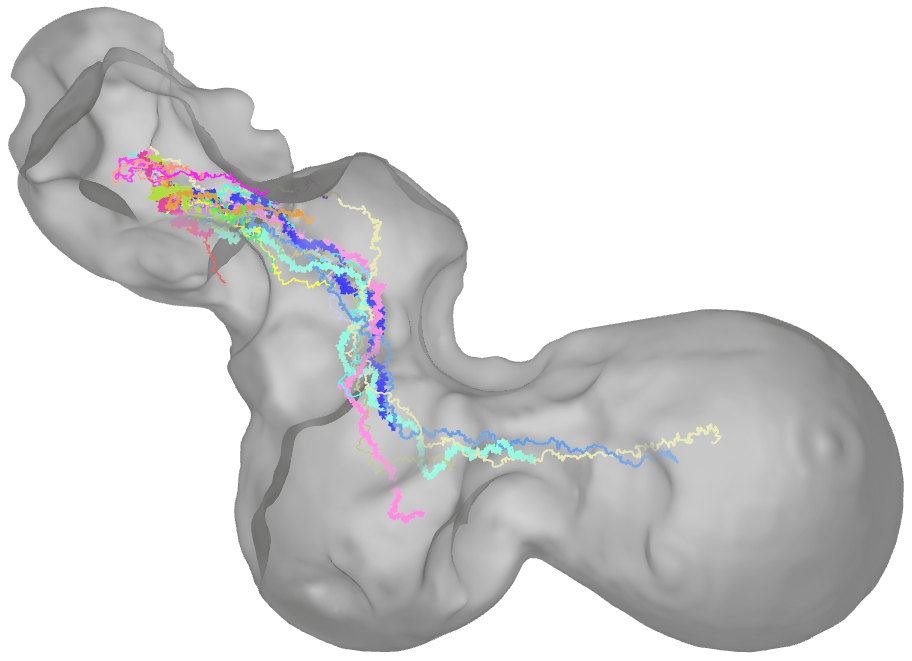
\includegraphics[width=0.45\textwidth]{fig/trajectories-clustered-21} \\
\end{tabular}
\caption{Visualization of resulting trajectories.
Left: All trajectories colored according to whether they reached the end of the tunnel (green) or they did not (red).
Right: Trajectories clustered according to their proximity colored by distinct colors.
The different line widths represent the number of trajectories in a cluster.}
\label{fig:trajectories}
\end{figure}

\section{Experimental verification}

The proposed method has been used to analyze a tunnel in Haloalkane dehalogenase (protein 1CQW) (Fig.~\ref{fig::tunnel}).
The tunnel was computed using CAVER 3.0~\cite{caver3} for spherical probe of radius 0.9~\AA.
The tunnel is represented by 760 spheres with average distance $0.05$~\AA.

% from David: m003 je "1-chlorpropan" a m004 "1-chlorbutan"
The traversability of the tunnel was evaluated for 1-chlorpropan (denoted as $\LA$) and 1-chlorbutan (denoted as $\LB$).

\begin{figure}
\centering
\caption{\label{fig::tunnel}
    TODO image of the tunnel + 1cqw
}
\end{figure}

\begin{table}
\centering
\caption{\label{tab::rrt}
    Runtime and sucess ratio of the planner
}
\input table.003.tex
\hskip 10pt
%\input table.004.tex
\end{table}



Further information can be found at {\url{http://mrs.felk.cvut.cz/isrr2017}}.

\section{Conclusion }


\section{Acknowledgments}

The presented work has been supported by the Czech Science Foundation (GA{\v C}R) under research project No. 17-07690S.
Access to computing and storage facilities owned by parties and projects contributing to the National Grid Infrastructure MetaCentrum, provided under the programme "Projects of Large Infrastructure for Research, Development, and Innovations" (LM2010005), is greatly appreciated.


\bibliographystyle{plain}
\bibliography{paper}

\end{document}











% ======================================================================
%
%    UNUSED TEXT      UNUSED TEXT      UNUSED TEXT     UNUSED TEXT
% ======================================================================




%RRT--Retraction~\cite{zhangRetraction} improves sampling in the narrow passages by retracting the newly added configuration
%closer to obstacles.
%%for motion planning of 3D objects.
%After $\qrand$ is generated and its nearest neighbor $\qnear\in \T$ is found, the segment from $\qrand$ to $\qnear$ is checked for collision.
%The tree is extended normally if the segment is free, otherwise the retraction step is performed.
%The task of the retraction step is to find a contact configuration  that minimizes the distance to $\qrand$.
%The contact configuration $q$ is found on the line and its neighborhood is searched to find another contact configuration $q'$ such that 
%$\varrho(q',\qrand) < \varrho(q,\qrand)$.
%The retraction is terminated after predefined number of steps or if no new contact configuration can be found.
%%The configuration trees built by RRT--Retraction can therefore contain more nodes than is the number of planning iterations,
%as the tree can be expanded by upto $\Nrret$ contact configurations in each iteration.
%An example of the retraction is depicted in Fig.~\ref{fig::rrtretraction}.
%The RRT-Retraction was designed for path planning of 3D objects, where the straight-line local planner is used to connect two configurations, which allows us to find the contact configurations by random sampling.
%The RRT--Retraction can quickly penetrate to narrow passages, but its computational burden is significantly
%increased due to necessity to find the contact configurations.
%The method was designed mainly for 3D path planning, but it can be combined with other planners
%for motion planning of many-DOF robots~\cite{pan2010retraction}.
%    e.g. for articulated robots~\cite{pan2010retraction}.
%RRT--Retraction combined with decomposition-based path planners for articulated robots with many DOF was proposed in~\cite{pan2010retraction}.

%The narrow passage problem has been studied intensively 
%Due to its low volume, the probability of expanding the nodes towards the passage is small~\cite{hannaWIS}.
%    many iterations are needed before a tree can be built through the passage~\cite{hannaWIS}.
%Recently, we have proposed a novel method for tunnel detection using sampling-based motion planning, namely using Rapidly Exploring Random Tree (RRT) method~\cite{vonasek2016application}.
%In comparison to existing approaches~\cite{Petrek20071357,petrek2006caver}, this RRT-based approach~\cite{vonasek2016application} 
%handles the dynamics without need to cluster and match Voronoi diagrams from consecutive frames.

%We further consider a spherical probe $\Sprobe$  of radius $\probe$ encapsulating the ligand.
%Let $q=(x,y,z)\in\C$ denote the configuration (position) of the probe, where
%the configuration space $\C$ consists of all possible configurations.
%For each configuration $q\in\C$ we assume, that its largest collision-free radius $r(q) \in \mathbf{R}, r(q)\ge 0$ can be computed, e.g.
%using collision detection.
%using collision detection.
%Let $L(q) \subseteq \mathbf{R}^3$ denote the geometry of the ligand at position $q \in \C$.
%Similarly to geometry of molecule, the geometry of ligand is union of hard sphere model.
%A probe is represented by one sphere of radius $\probe$.
%The collision-free region $\CF \subseteq \C$ is formed by configurations, where $\Sprobe$ can be placed without any collision, i.e., 
%$\CF = \{q \in \C | \Sprobe(q) \cap \SS = \emptyset\}$, where $\Sprobe(q)$ is the sphere with radius $\probe$ at configuration $q$.
%The distance $\dist(q_1,q_2)$  between two configurations $q_1,q_2\in\C$ is measured using 3D Euclidean metric.

%This radius can be detected using collision detection method.
%The configurations outside the protein $\CG \subseteq \C$ are collision-free with sphere $\Sgprobe$ of radius $\gprobe$, $\gprobe> \probe$,
%$\CG=\{q\in \C| \Sgprobe(q) \cap \SS = \emptyset \}$.
%A configuration $q \in \CG$ is referred to as {\sl goal configuration} in the rest of the paper.
%By computing $\alpha$-shape of the molecule, we can identify atoms located at the surface. 
%These atoms are referred to as {\sl surface atoms} in the rest of the paper.
%The distance between a configuration $q \in \C$ and its nearest surface atom is referred to as $\dists(q)$.
%We assume, that for each configuration $q$, the largest collision-free radius $r(q)$ can be computed.
%Let $r(q)$ denote the radius of the largest collision-free sphere at configuration $q$.

%Dynamic proteins are represented by a sequence of $n$ snapshots (frames).
%The tunnels change with the protein dynamics as well: their width and position change, they can merge with other tunnels or even disappear.
%The free region $\CF$ is therefore different in each frame, as positions of atoms change.
%For the sake of simplicity, a single notation $\C$ resp. $\CF$ is used in this paper and it is valid for the frame being processed.

%Approximated WVD diagram of the atoms is computed by representing each atom using 12 balls of equal radii and computing ordinary Voronoi diagram.
%Computing WVD this way is more efficient and numerically stable and it is used also in other related tools~\cite{caver3,yaffe2008}.
%Vertices of this WVD are filtered out if their distance to an atom is less than probe radius $\probe$.
%Let $\VV$ contain the remaining Voronoi vertices, and let $r_v \in \VV$ denote the distance to the nearest atom.
%The remaining Voronoi vertices $\VV$ of the WVD and their distances $r_v, v\in \VV$ to the nearest atom are then used in the following method.

%A possible solution is to estimate the location of narrow passages from the knowledge of the workspace and generate more samples in the difficult areas.
%For Probabilistic Roadmaps~\cite{kavrakiPRM}, this can be achieved simply by generating more samples in the difficult areas, e.g. along
%medial axis~\cite{wilmarthMAPRM,foskey01hybrid,guibas1999probabilistic,hoff2000interactive,yang2004adapting}.
%This requires to precompute the medial axis, which can be time consuming.
%Another approach is to shift the random samples towards the medial axis~\cite{amatoOBPRM} or into a direction of estimated
%medial axis~\cite{hollemanMAPRM}.
%Generating random samples in difficult regions however does not ensure construction of a better tree in the case of RRT-based methods. 
%In RRT, the configuration tree is expanded in the direction of random samples, but the obstacles may prevent to reach them closely~\cite{vonasekphd}.
%Increased probability of sampling in a given region, e.g., in a narrow passage, 
%brings advantage only if the tree is close to the region and if it can reach it.
%it is necessary to maintain the sampling regions according the progress of the tree.
%For example, random samples can be generated along a given workspace path~\cite{vonasek2009rrt}.
%After the tree reaches a path point, the sampling around the point is disabled and moved to the next point of 
%the path.
%Similar approach is used in~\cite{denny2014marrt}, where the sampling regions are maintained with a grapth describing topology 
%of the workspace.
%OB-RRT~\cite{amatoOBRRT} defines several types of tree expansions
%steps based on information about obstacles (e.g. using vectors of obstacles, tangential vectors and information about medial axis).

%~\cite{amatoOBPRM,hollemanMAPRM} shift random samples towards medial axis of the environment, which helps to sample
%narrow passages more densely. 
%For example, the random samples generated in the configuration space can be shifted
%towards the medial axis of the environment~\cite{amatoOBPRM,hollemanMAPRM} or even generated around the medial 
%axis~\cite{wilmarthMAPRM,foskey01hybrid,guibas1999probabilistic,hoff2000interactive,yang2004adapting}.
%The paper~\cite{amatoOBPRM} suggests to sample uniformly in the configuration space and shift the samples towards the medial axis.
%Another approach is to generate the samples randomly in \CS\ and shift them closer to the medial axis~\cite{amatoOBPRM}.
%The medial axis can be computed exactly using GVD.
%While the medial axis can be easily computed for 2D or 3D workspaces using GVD, its computation become complicated in many dimensions.
%In such case, the samples can be generated uniformly from the whole \CS\ and moved in an estimated direction towards the medial axis~\cite{hollemanMAPRM}.



%sampling-based for 
%protein-ligand access and docking \cite{bayazit2001ligand,singhLig,apaydin2004stochastic,cortes2010simulating}
%protein and RNA folding~\cite{amatoPF1,ApaBru03}
%protein loop motions~\cite{cortes2004geometric},
%domain motions~\cite{kirillova2008an}, 
%and motions of pairs of alpha-helices in transmembrane proteins~\cite{enosh2007prediction}

%The tree is extended from a node, that is selected as a nearest node to a randomly generated configuration in the configuration space.
%The highest probability of expansion have nodes with large Voronoi cells. 
%Due to this Voronoi-bias, the tree grows towards unexplored regions of the configuration space.
%However, the Voronoi-bias brings disadvantages in narrow passages.
%nodes in the narrow passages.



%The behavior of RRT in the narrow passages was analyzed using Voronoi diagrams in~\cite{yershovaDDRRT}.
%The nodes in the tree can be divided into two groups: frontier nodes, whose Voronoi cells grow together with growth
%of the environment and boundary nodes, which are close to the obstacles. %~\cite{yershovaDDRRT}.
%The tree cannot be expanded from the boundary nodes.
%In a narrow passage, the nodes are both boundary and frontier.
%These nodes are frequently selected for the expansion, because they are the frontier nodes, however the tree cannot be expanded
%from them, because they are also the boundary nodes. 
%To suppress selection of the boundary nodes, authors of~\cite{yershovaDDRRT} suggest to define an action radius around each node.
%The node is selected for the expansion only if its radius is larger than the distance to the random sample.
%The radius of new nodes is set to $\infty$ and it is decreased to a predefined value $\rdd$ if the node cannot be expanded.
%A Dynamic-Domain strategy for RRT (RRT--DD) is proposed in~\cite{yershovaDDRRT}:
%each node holds an action radius defining how far can be a random sample $\qrand$ that activates the node for the expansion.
%The RRT--DD algorithm generates random samples $\qrand$  and finds its nearest neighbor in the tree
%$\qnear$ until $\rho(\qrand,\qnear) < \qnear.radius$. 
%Although the algorithm is efficient in the narrow passages, it is strongly influenced by the parameter $\rdd$.
%To decrease the sensitivity of the method to the parameter $\rdd$, it can be automatically adjusted, which
%was proposed in RRT--ADD (RRT with Adaptive Dynamic Domain)~\cite{jailletATDDRRT}.
%Another schema to automatically adjust parameters of the RRT-based planners was proposed in~\cite{schneider2015completely}.

%Retraction-RRT~\cite{zhangRetraction} generates random samples uniformly as in the original RRT, but it
%attempts to shift them into the narrow passages.
%A~random configuration $\qrand \in \CF$ is generated and a close non-free configuration $q \in \CO$ is found. 
%A~contact configuration $q_c$ on a segment $(\qrand,q)$ is found and its neighborhood is searched for
%$q_c'$ minimizing the distance between $q$ and $q_c'$. 
%The configuration $q_c'$ is then added to the tree.
%It was shown that this approach can deal with narrow passages efficiently,
%because the generated contact configurations penetrate into the narrow passages.
%However, to find the contact configurations, the collision detection algorithm is called frequently, which can decrease
%the performance of the algorithm.

%The goal-bias principle can be further extended by sampling the configuration space along a path computed in the workspace~\cite{vonasek2009rrt,amatoOBRRT}.
%%Geometric path in the workspace~\cite{vonasek2009rrt} or medial axis of the 3D space~\cite{amatoOBRRT} can be used to guide the tree.
%Sampling along geometric paths constructed in the workspace is suitable for low-dimensional configuration spaces, e.g. for
%path planning of mobile robots.
%However, the geometric paths computed in workspace are less effective for sampling in high-dimensional configuration spaces~\cite{hannaWIS}.
%



%of the narrow passages is related to narrow passaged of the workspace~\cite{hannaWIS}.
%
%is to manipulate the random samples, e.g. to change their rotation, rotation or both parts or to shift them closer to the medial
%axis of the workspace~\cite{amatoOBPRM}.

%In~\cite{amatoOBPRM} several strategies for validating non-free random samples have been proposed.
%Authors propose different manipulation procedures for random configurations generated during the learning phase.
%For example, the random configuration can be placed into the roadmap with changed rotation, translation or both, or it can be
%shifted away from an obstacle allong a line connecting the sample and medial axis of the obstacles.
%In a configuration is invalid, it is pushed randomly into various directions to gen free samples around boundaries of $\CO$.





% ===============================================================================


%25\% of VDW radii, T-RRT \cite{jaillet10costmap}

%\red{The tunnel detection task differs from classic motion planning it two main aspects: a) the goal configuration
%is not explicitly defined, and b) multiple pathways (tunnels) should be detected.}


%Molecular structures can be represented as articulated bodies and sampling-based methods can be used
%Path planning methods have been used to expore the conformational space of 
%proteins~\cite{novinskaya2015improving,songPFintro,mollProt,proteinRRT},
%Other applications of sampling-based approaches is in detection of 
%folding pathways~\cite{amato2002using}, analyzing protein loops~\cite{cortes2004geometric}, 
%or modeling large-scale transitions in a protein structure~\cite{raveh2009rapid}
%The geometric-based tunnel detection approaches provide fast computation of tunels in large protein structures and they
%have been integrated in several tools like Caver~\cite{bara2014caver}, Chexvis~\cite{masood2015chexvis} and other.
%Most of the proposed methods consider only spherical models of ligand~\cite{benkaidali2014computing}.

%dxTuber: Detecting protein cavities, tunnels and clefts based on protein and solvent dynamics:
%furtng protein cavities, tunnels and clefts based on protein and
%solvent dynamics insights into the protein in question. For example, empty
%space in a protein structure can provide valuable insight into protein properties such as internal hydration, structure stabilization,
%substrate translocation, storage compartments or substrate binding sites [1,2]. This information can be visualized by means of cav-
%ity analysis. Over the years numerous cavity detection tools have been developed including [3–17] that depict cavities either directly
%[3–6,8,10–17] or indirectly by identifying lining residues [9] or filling a cavity with water molecules [7]. The main strategies used
%in these geometry-based algorithms [1] can be grouped into four categories plus combinations of these.
%n the motion planning problem, that is widely studied in robotics, the task is to find a feasible trajectory for a robot between two

%given positions in an enironment.
%To utilize the motion planning approaches, the ligand is considere as the robot and the protein's atoms as the obstacles.
%Computing feasible (traversable) tunnels for non-spheric ligands requires to consider also rotations of the ligands, which 
%can be solved using sampling-based approaches like Probabilistic Roadmaps (PRM)~\cite{kavrakiPRM} or Rapidly Exploring
%Random Trees (RRT)~\cite{lavalleRRT}.
%Sampling-based methods randomly samples configuration space of the robot (ligand) and the samples are classified
%as free or non-free using collision detection.
%The free samples are stored in a graph structure.
%A path in the grap then corresponds to a motion in the workspace.



%In~\cite{guieysse2008structure}, RRT method is used to compute pathways for flexible ligands.


%\cite{lindow2012dynamic}
%Analysis of protein dynamics suggests that internal cavities and channels can be rather dynamic structures. 
%Voronoi-based algorithm to extract the geometry and the dynamics of cavities and channels from a molecular dynamics trajectory.
%The algorithm requires a pre-processing step in which the Voronoi diagram of the van der Waals spheres is used to calculate the cav-
%ity structure for each coordinate set of the trajectory. 
%In the next step, we interactively compute dynamic channels by analyzing the time evolution of components of the cavity structure. Tracing of the
%cavity dynamics is supported by timeline visualization tools that allow the user to select specific components of the cavity structures
%for detailed exploration. All visualization methods are interactive and enable the user to animate the time-dependent molecular struc-
%ture together with its cavity structure. To facilitate a comprehensive overview of the dynamics of a channel, we have also developed a
%visualization technique that renders a dynamic channel in a single image and color-codes time on its extension surface. 
%
%
%Sampling-based motion planning algorithms from the field of robotics have been very successful in exploring the
%conformational space of proteins
%\cite{novinskaya2015improving}
%Sampling-based algorithms explore the conformational space of a protein by randomly sampling it (usually using a special
%heuristic) and constructing a graph where each node represents a feasible low-energy protein conformation (or state), and each
%edge represents a possible low-energy local transition between two states. 
%The computed graph describes the topology of a protein’s energy landscape and the connectivity of its lowenergy areas. 
%This graph can be used to find possible large-scale transitions between two given protein conformations.
%

%Sampling-based methods have been very effective for the fast computation of representative motions of molecular systems \cite{al2012motion, gipson2012computational}


%A broad range of approaches exploit sampling-based techniques to address various biological problems, such
%as exploring energy landscapes \cite{devaur2014sampling} ,
%modeling protein folding pathways \cite{amato2002using}, analyzing protein loops \cite{cortes2004geometric}, 
%or modeling large-scale transitions in a protein structure \cite{raveh2009rapid}

%In computational biology, molecules and proteins are modeled as articulated bodies and sampling based planners are used to simulate
%protein folding and protein-ligand interactions  \cite{al2012motion} 
%asi spis necitovat \cite{gipson2012computational}



%Ms have been applied to model molecular motions by modeling the molecule as an articulated linkage and 
%replacing the typical collision detection validity check with some measure of physical viability (e.g., potential energy).
%Protein motions, ranging from molecular flexibility to large-scale conformational change, play an essential role in many biochemical processes. 
%!!to map transitinos between specific conmfotrmations!!!!
%ample conformation space more effectively, and we describe extensions of our framework to automate
%the process and to map transitions between specified conformations.
%\cite{thomas2006simulating}
%

%In subsequent work, our group used another PRM variant on this problem \cite{bayazit2001ligand}
%Our group was the first to adapt PRMs to model protein folding pathways 
%\cite{amato2003using, amato2002using, song2003apath}

%Using a standard modeling assumption for proteins that bond angles and bond lengths are fixed \cite{sternberg1996protein}, 
%the only dof in our model are the backbone’s phi and psi torsional angles which are modeled as revolute joints with values 0 .. 2pi

%
%The roadmap produced by our technique is an approximation of the protein’s energy landscape. 
%Roadmap quality is measured both by how realistic (as compared to experimental data) its pathways are and by how many samples are required
%to achieve the desired accuracy. 
%The latter is important because it determines what size molecules can be analyzed.
%Hence, sampling is the key to producing a good approximation of the land-scape. 
%Note that only a relatively small portion of the conformation space ‘near’ the target conformation(s) is of interest in modeling motions. 
%This implies that we should use biased sampling to cover the regions of interest efficiently.
%
%genrovani lepsich vzorku: using rigidity analysis~\cite{thomas2006simulating}
%or perturbing:
%iterative sampling process where we apply small Gaussian perturbations to existing conformations~\cite{amato2003using, amato2002using, song2003apath}
%
%rrt for tunnel (pathway) detection
%\cite{cortes2010simulating}
%\cite{corset2005path}
%\cite{guieysse2008structure}
%

%Many modifications have been proposed for RRT to speed up the growth of the tree~\cite{kuffnerRRTC}, 
%     to consider an optimality criteria such as path length~\cite{karaman2011sampling}, and to improve behavior in narrow passages~\cite{amatoOBRRT,vonasek2009rrt,zhangRetraction,schneider2015completely}. 
%For example, RRT--Retraction~\cite{zhangRetraction} analyzes the line segment from $\qnear$ to $\qrand$.
%If the line segment is collision-free, the tree is expanded normally using the straight-line planner.
%Otherwise, the contact configuration on the line segment is constructed and its neighborhood is searched
%for other contact configurations in order to minimize the distance to $\qrand$.
%This retraction step allows RRT--Retraction to place the nodes of the tree into narrow passages.



%The behavior of RRT in the narrow passages was analyzed using Voronoi diagrams in~\cite{yershovaDDRRT}.
%The nodes in the tree can be divided into two groups: frontier nodes, whose Voronoi cells grow together with growth
%of the environment and boundary nodes, which are close to the obstacles. %~\cite{yershovaDDRRT}.
%The tree cannot be expanded from the boundary nodes.
%In a narrow passage, the nodes are both boundary and frontier.
%These nodes are frequently selected for the expansion, because they are the frontier nodes, however the tree cannot be expanded
%from them, because they are also the boundary nodes. 
%To suppress selection of the boundary nodes, authors of~\cite{yershovaDDRRT} suggest to define an action radius around each node.
%The node is selected for the expansion only if its radius is larger than the distance to the random sample.
%The radius of new nodes is set to $\infty$ and it is decreased to a predefined value $\rdd$ if the node cannot be expanded.
%A Dynamic-Domain strategy for RRT (RRT--DD) is proposed in~\cite{yershovaDDRRT}:
%each node holds an action radius defining how far can be a random sample $\qrand$ that activates the node for the expansion.
%The RRT--DD algorithm generates random samples $\qrand$  and finds its nearest neighbor in the tree
%$\qnear$ until $\rho(\qrand,\qnear) < \qnear.radius$. 
%Although the algorithm is efficient in the narrow passages, it is strongly influenced by the parameter $\rdd$.
%To decrease the sensitivity of the method to the parameter $\rdd$, it can be automatically adjusted, which
%was proposed in RRT--ADD (RRT with Adaptive Dynamic Domain)~\cite{jailletATDDRRT}.
%Another schema to automatically adjust parameters of the RRT-based planners was proposed in~\cite{schneider2015completely}.

%Retraction-RRT~\cite{zhangRetraction} generates random samples uniformly as in the original RRT, but it
%attempts to shift them into the narrow passages.
%A~random configuration $\qrand \in \CF$ is generated and a close non-free configuration $q \in \CO$ is found. 
%A~contact configuration $q_c$ on a segment $(\qrand,q)$ is found and its neighborhood is searched for
%$q_c'$ minimizing the distance between $q$ and $q_c'$. 
%The configuration $q_c'$ is then added to the tree.
%It was shown that this approach can deal with narrow passages efficiently,
%because the generated contact configurations penetrate into the narrow passages.
%However, to find the contact configurations, the collision detection algorithm is called frequently, which can decrease
%the performance of the algorithm.


%Another approach to biased sampling was presented in~\cite{bruceERRT}, where the trajectories found in previous
%iterations are used to sample the configuration space. 
%This modification is suitable for dynamic environments.

%The growth of the tree can be attracted into a region $\R \in \C$ by increasing probability of sampling in that region.
%This is used in the goal-bias principle~\cite{lavalleRRTPP}, where $\qgoal$ is used instead of $\qrand$ with the probability $\gb$.
%The goal-bias suppresses the exploration of $\C$ and the tree is expanded more preferably towards the goal.
%An extension of the goal-bias was presented in~\cite{kardossRRTKK}, where a predefined key-configuration is 
%used to focus sampling to difficult areas of the configuration space.
%%Authors suggest to place the key-configuration in a way that connects easy and difficult areas of the configuration space.
%%For example, the key-configuration can be placed at the enter to a narrow passage.
%%Although the goal-bias speeds up the growth towards the goal, it may cause a congestion problem of the tree growth due to existence of an obstacle in the pathway.
%
%
%The goal-bias principle can be further extended by sampling the configuration space along a path computed in the workspace~\cite{vonasek2009rrt,amatoOBRRT}.
%%Geometric path in the workspace~\cite{vonasek2009rrt} or medial axis of the 3D space~\cite{amatoOBRRT} can be used to guide the tree.
%Sampling along geometric paths constructed in the workspace is suitable for low-dimensional configuration spaces, e.g. for
%path planning of mobile robots.
%However, the geometric paths computed in workspace are less effective for sampling in high-dimensional configuration spaces~\cite{hannaWIS}.
%

%deformable objects in many fields like computer graphics, robotics and medicine~\cite{alterovitz2008motion} clothing, rope, human tissue
%a two-stage approach was presented in~\cite{bayazit2002deformable}. 
%First a path is found with reduced-scale of the robot, or by allowing the robot to penetrate obstacles.
%The roadmap can therefore contain configurations that are infeasible for the rigid version of the robot
%After finding a path, the infeasible configuraions are determined and the robot is deformed there to avoid the collisions.
%the path is refined to remove the collisions
%geometric deformation -- only part of the object that is colliding is deformed,
%and bounding box (first bounding box is deformed and the the model is deformed according to the deformation compute for the bbox)
%path planning with non-rigid obstacles~\cite{frank2008efficient}.

%the majority of path planning approached focus on rigid robots and rigid obstacles.
%\cite{gayle2005path},planning for a flexible robot in complex environments. 
%algorithm  computes a collision free path by taking into account geometric and physical constraints, including obstacle avoidance, non-
%penetration constraint, volume preservation, surface tension, and energy minimization. 

%new algorithm for collision detection between a deformable robot and fixed obstacles using  graphics processors. 
%We also present techniques to efficiently handle complex deformable models composed of tens of thousands of polygons and obtain significant performance improvement    over previous approaches. 
%practical application of our algorithm in performing path planning of catheters in liver chemoembolization.
%planning for flexible objects~\cite{lamiraux2001flexible}, 
 
% f-PRM \cite{kavraki1998towards} framework for flexible robots of simple geometrix shapes\cite{anshelevich2000deformable} or surface patches~\cite{holleman1998planning}.

%other planning for defomrable: \cite{anshelevich2000deformable,bayazit2002deformable,gayle2005path}
%deformable envinorments: \cite{rodriguez2006planning,frank2008efficient,phillips2014representation}

%representation of deformation~\cite{phillips2014representation}

%Robots can be deformed either considering their physical propersites or not.
%geometrical or physical-based deformation approaches
%The non-physical deformations include basic deformations  like scale, bend or twist~\cite{barr1984global},
%   free-form deformation~\cite{gibson19973d,sederberg1986free},
%   Physical-based deformations can be achiebed using mass-spring and finite-element methods.
%f-PRM~\cite{anshelevich2000deformable}, physically coreect deformations, time consuming




